
\chapter{Software Architecture and Simulation Environments}

This chapter discusses the software architecture of the mobile manipulation system and the simulation 
environments used for testing and development. The software architecture is based on the Robot Operating System 2 (ROS2)
middleware, which provides a flexible and modular framework for developing robotic applications. 
The simulation environments are based on Rviz2 and Ignition Gazebo, which provide realistic simulation environments
for testing algorithms before deployment.

\section{ROS2 Control Interface for Igus Rebel Arm}
\label{sec:ros2control}

The first step in developing the software architecture for the mobile manipulator is to interface the
Igus Rebel Arm with ROS2. The Igus Rebel Arm is a 6-DOF robotic arm that can be controlled by either the CAN binary bus
or the Ethernet interface (proprietary CRI protocol). The CAN bus interface is used for low-level access to the arm's
joints, while the Ethernet interface is used for high-level control and monitoring of the arm's state. 
The ROS2 control interface for the CAN bus was already implemented by the control software provider \textit{Commonplace Robotics}.
However, this type of connection requires a proprietary cable. Moreover, an Ethernet connection is more flexible, since the manipulator can be connected to the switch and controlled by any computer on the local network.

Developing the \textbf{ROS2 control interface} for the Ethernet interface required understanding the \textbf{CRI protocol},
which is a protocol based on plain text messages. The CRI protocol is used to send commands to the arm in the form of
joint positions (i.e. rotation of the motors in radians) or velocities (i.e. jogs) 
and to receive feedback from the arm in the form of joint positions (values provided by the motors' encoders).
The Igus Rebel cobot provides a \textit{Raspberry Pi} embedded computer that runs the control software for the arm's motors
and acts as the CRI server, which listens for commands on the Ethernet interface and sends feedback to the client.
The CRI client is the ROS2 control interface, while the CRI server acts as a bridge between the arm's motors embedded
closed loop motor driver controllers and the control software (either the software provided by the manufacturer or
the ROS2 control interface).

Controlling the cobot using ROS2 requires a hardware interface, used to command and control the robot by interfacing
with the CRI communication protocol. ROS2-Control is the framework provided with ROS2 that makes it possible to develop such
hardware and control interfaces. The hardware interface is implemented as a ROS2 lifecycle node that
is interfaced directly with the Joint Trajectory Controller, which is a ROS2 controller that can be used to
control the arm using joint trajectory messages, containing the desired joint positions or velocities.
While the Joint Trajectory Controller is a standard robot controller provided within ROS2-Control that can work
with any robot arm and configuration, the hardware interface was developed and implemented specifically for the Igus Rebel Arm
and its CRI communication protocol. The implementation of the hardware interface is based on the \textit{System Interface}
provided by ROS2-Control, which is a type of interface that supports joints and actuators. The System Interface
accesses the hardware via the CRI protocol and is managed by the Controller Manager and the Resource Manager.

The Joint Trajectory Controller is then handled by MoveIt2, which is a ROS2
motion planning framework that can be used to plan and execute trajectories for the arm \cite{moveit2}.
\textbf{MoveIt2} generates motion plans for the robot using the robot's kinematic model and the obstacles in the environment.
The Joint Trajectory Controller receives the computed trajectories from MoveIt2 and sends them to the arm 
using the hardware interface.

%Add a Figure of the control architecture
\begin{figure}[t]
    \centering
    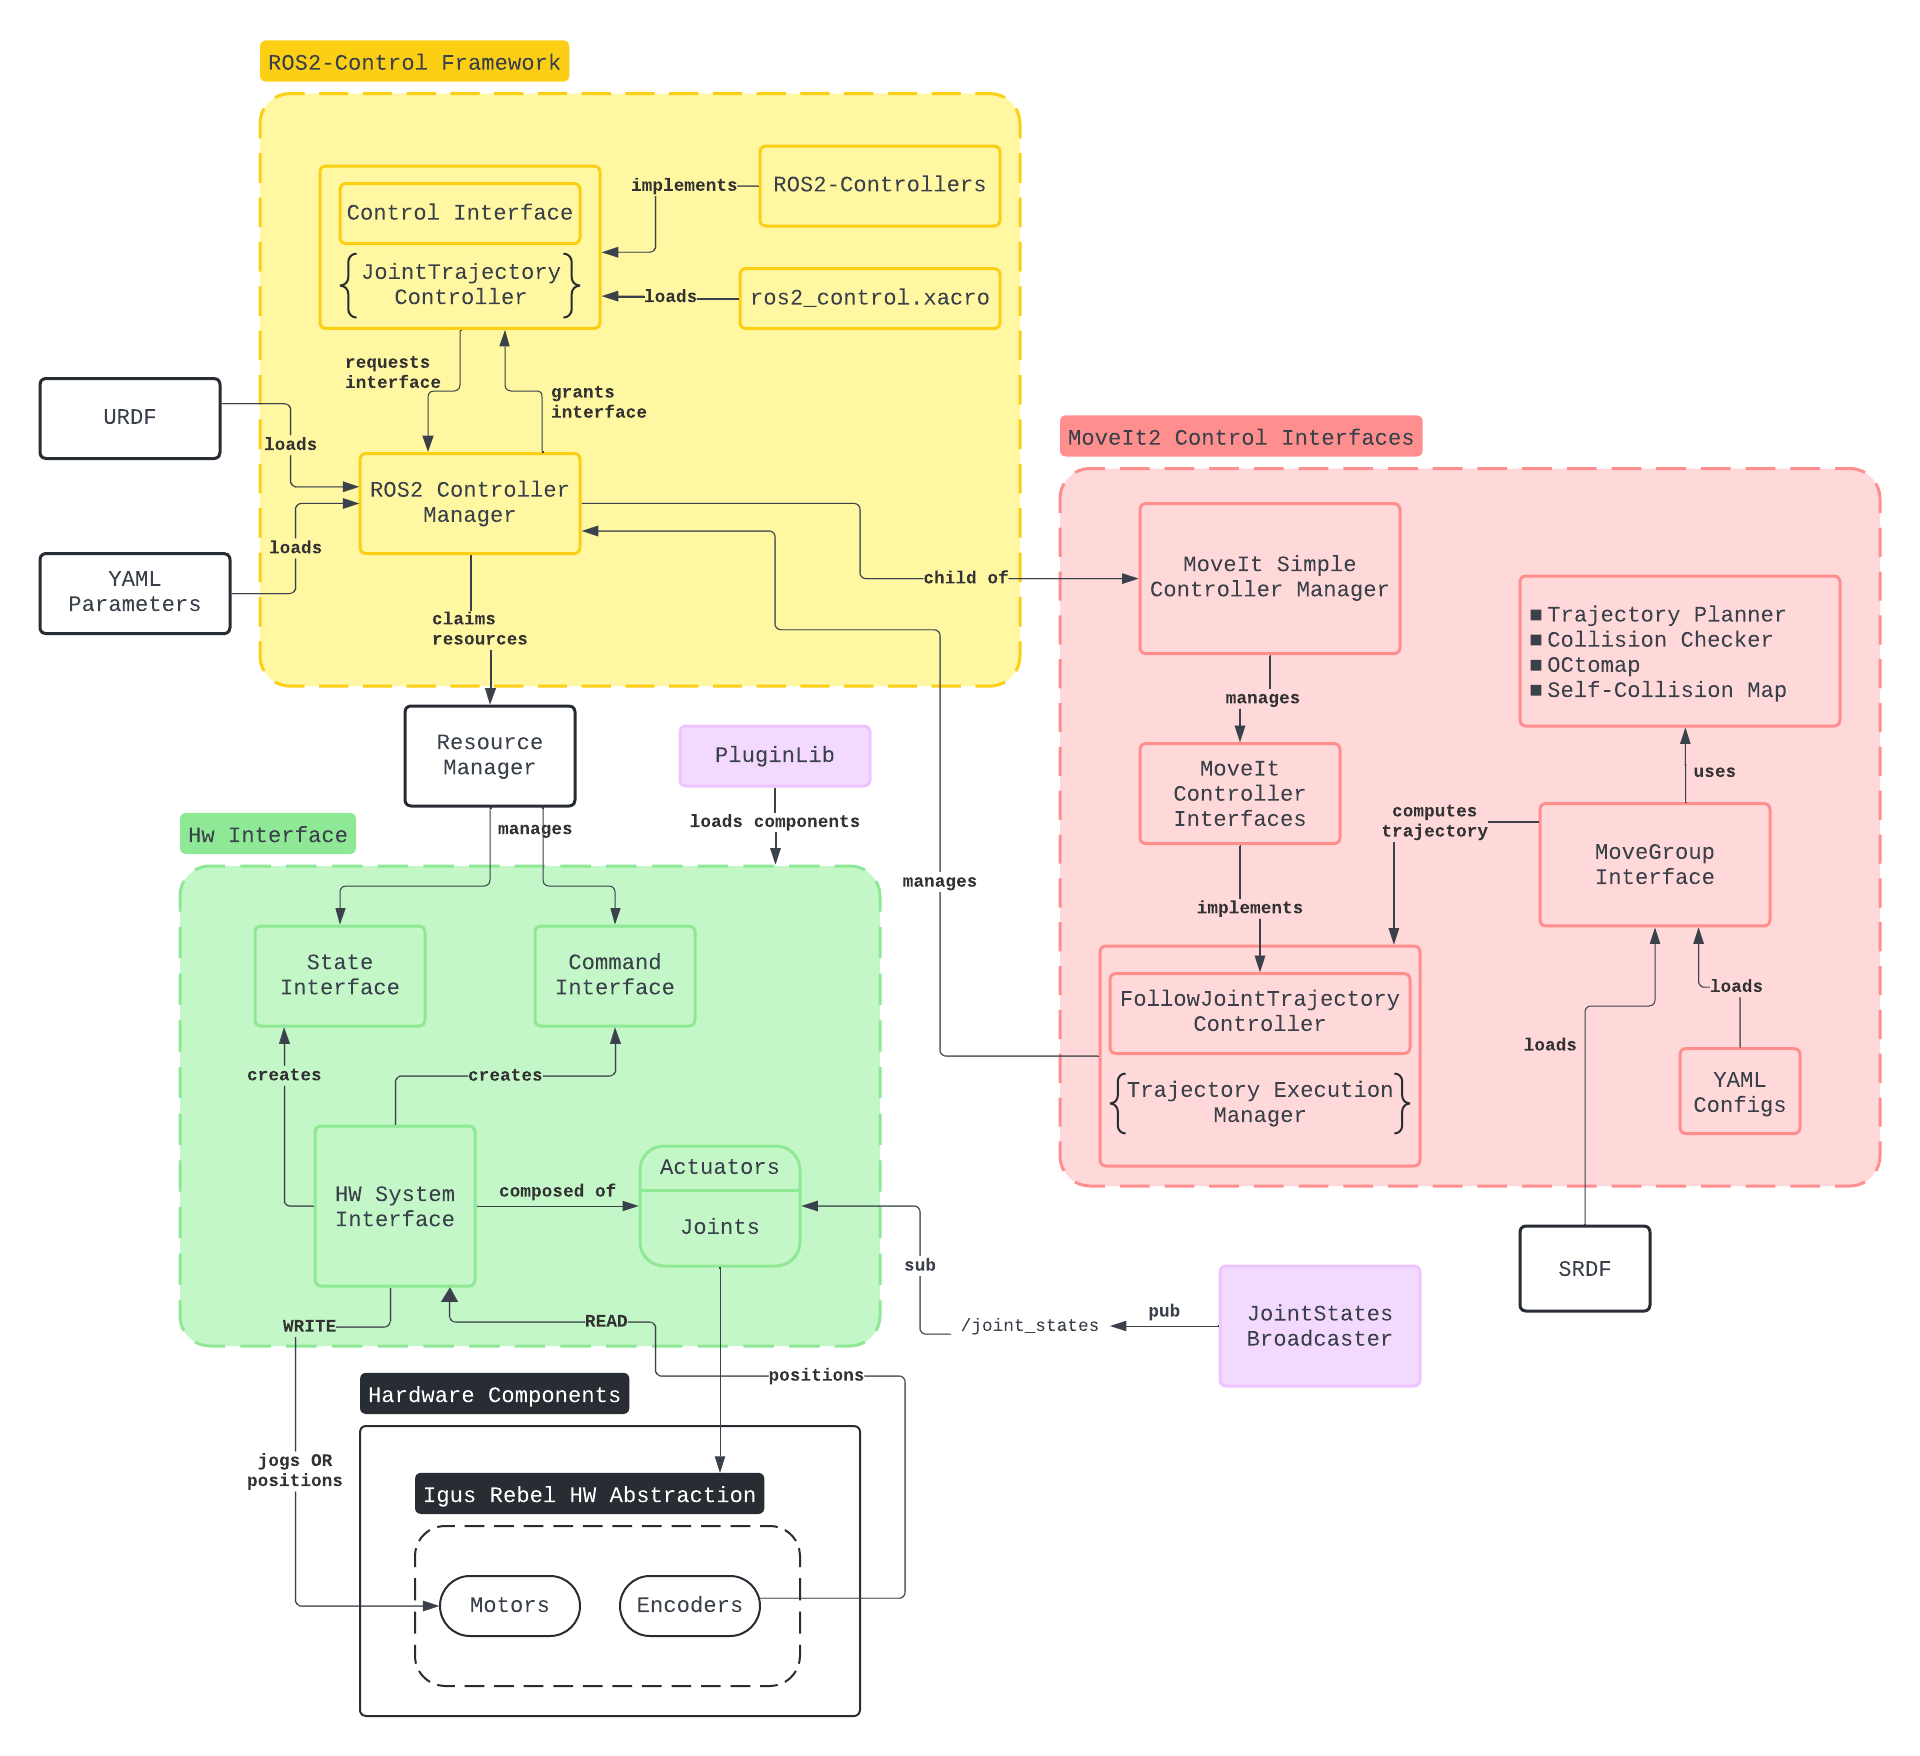
\includegraphics[width=1.0\textwidth]{ros2 control architecture_updated.png}
    \caption{ROS2-Control and MoveIt2 Interfaces Architecture}
    \label{fig:ros2control}
\end{figure}

The diagram in Figure \ref{fig:ros2control} shows an overview of how the implemented ROS2 hardware interface works,
and how it is connected to the ROS2 Controller and MoveIt2 motion planners. The hardware interface relies on the
hardware components abstraction layer, a set of classes that provide an interface to the hardware components
of the robot, such as the arm's motors and encoders. The state interface is used to read the state of the robot's joints
(reads the position values from the motors' encoders), while the command interface is used to send commands to the robot's
joints (sends the desired joint positions or velocities to the motors).
The diagram also shows the connection between the ROS2 Controller Manager and the MoveIt2 controller managers,
which are responsible for managing the execution of the trajectories generated by MoveIt2's planners and sending commands
to the appropriate ROS2 controllers based on the desired robot motion. The \textit{FollowKJointTrajectoryController}
is the interface for the underlying action server that sends the joint trajectories to the Joint Trajectory Controller.

Integrating the MoveIt2 libraries with the ROS2 framework requires MoveIt2 controller managers, 
a set of controllers that can be used to control the robot's motion.
MoveIt2 controller managers act as the bridge between high-level motion planning in MoveIt2
and the low-level control of robot hardware. They are responsible for managing the execution of trajectories
generated by MoveIt2's planners, sending commands to the appropriate ROS2 controllers based on the desired robot motion.
These ROS2 controllers such as the Joint Trajectory Controller, in turn, interact with the hardware interfaces 
to translate the control commands into actions that the robot can execute. This \textbf{layered architecture}
allows for modularity and flexibility in the robot control system, enabling the integration of various controllers
and hardware interfaces without affecting the high-level motion planning capabilities of MoveIt2.
\textit{MoveItSimpleControllerManager} is the controller manager used with MoveIt2 to control the robotic arm
using the Joint Trajectory Controller and the \textit{FollowJointTrajectory} action for sending motion execution goals.

\subsection{Joint Trajectory Controller}

The Joint Trajectory Controller is a ROS2 controller that can be used to control the arm using joint trajectory messages.
These messages are joint-space trajectories on a group of joints.
The controller interpolates in time between the points so that their distance can be arbitrary. 
Trajectories are specified as a set of waypoints to be reached at specific time instants, which the controller 
attempts to execute as well as the underlying hardware allows.
Waypoints consist of either positions or velocities, accelerations are optional.

The Joint Trajectory Controller can be operated either in position, velocity, or acceleration mode, 
depending on the type of trajectory message that the hardware interface can handle.
The position mode is used to send joint positions to the arm, while the velocity mode is used to send joint velocities
in the form of jog values (i.e. velocities in percentage of the maximum velocity). The Joint Trajectory Controller can
be operated either in closed-loop or open-loop mode, depending on the presence of the feedback that is used to control the arm.
In closed-loop mode, the controller uses the joint positions received from the arm as feedback to adjust the trajectory
to the desired position, by controlling the arm via velocity commands. In open-loop mode, the controller sends the
trajectory to the arm without any feedback, which can be useful for testing the arm's performance without any feedback
control.

The closed-loop velocity control requires a \textbf{PID controller} to adjust the velocity commands based on the
difference between the desired and actual joint positions. The PID controller requires tuning the gains to
achieve a stable and smooth trajectory execution. Tuning the gains is a challenging task that requires
either the system's model or a realistic simulated robot model that mimics the real robot's behavior and dynamics.
Moreover, this is a time-consuming task that requires extensive testing with many trials and errors to find the best gains 
for the PID controller. Insufficiently tuned gains can lead to strong oscillations in the joint positions and the arm
not reaching the desired pose stably. In the worst case, the arm can collide with obstacles in the environment
or even damage itself. In the case of the Igus Rebel Arm, it was not possible to carry out the PID gains tuning
due to the lack of a realistic simulated robot model and the impossibility of testing the dynamics and impulse responses
of the robotic arm in a safe environment. Therefore, the open loop controller was used throughout the project.

\section{MoveIt2 and RViz2 Simulation Environment}

% Add a Figure of the MoveIt2
\begin{figure}[t]
    \centering
    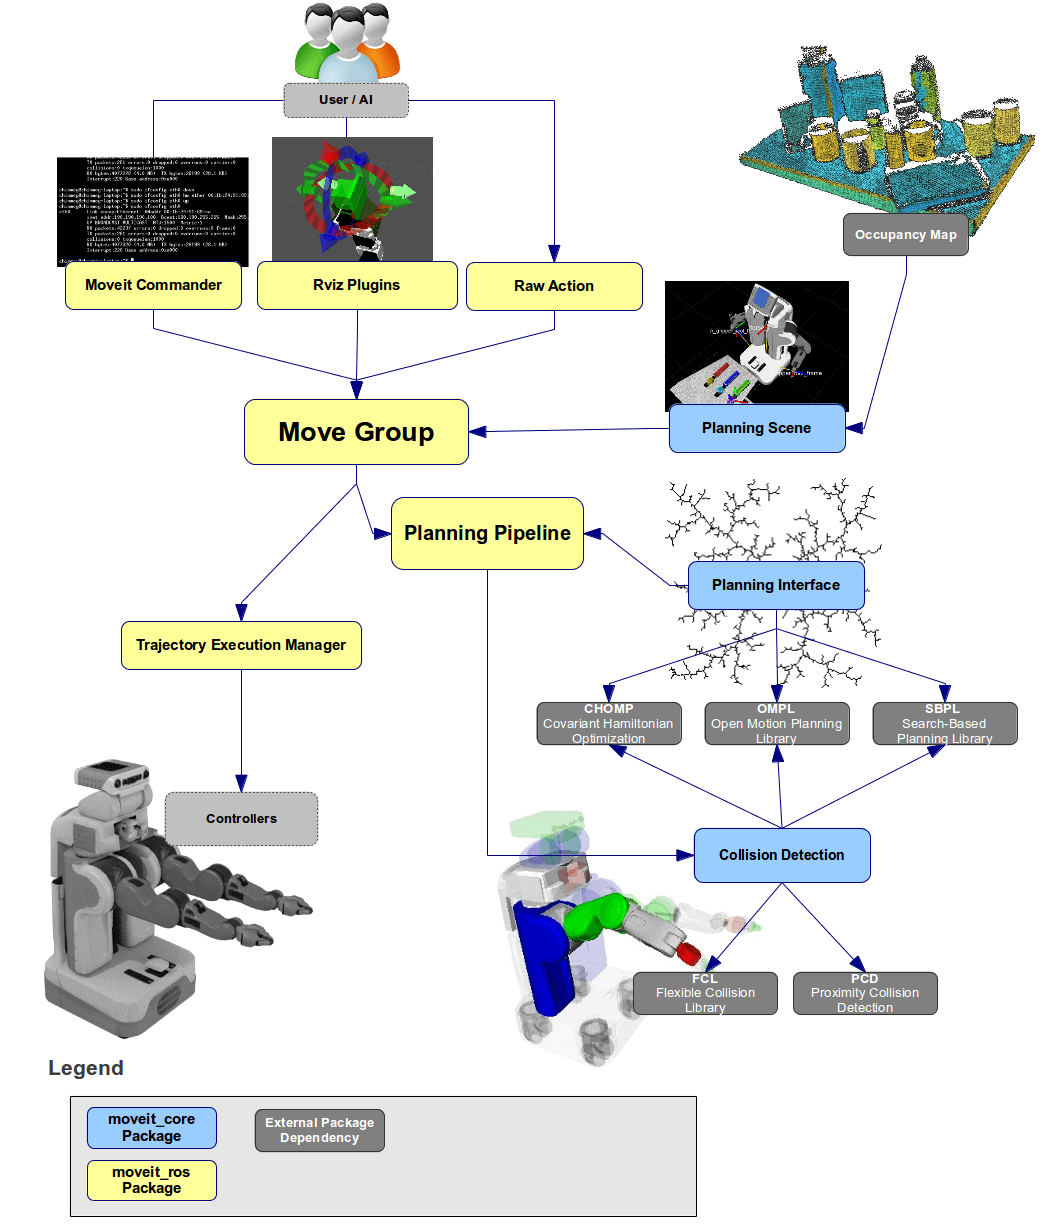
\includegraphics[width=0.8\textwidth]{c4_01.png}
    \caption{MoveIt2 General Architecture}
    \label{fig:moveit2}
\end{figure}

%Add a Figure of the control architecture
\begin{figure}[t]
    \centering
    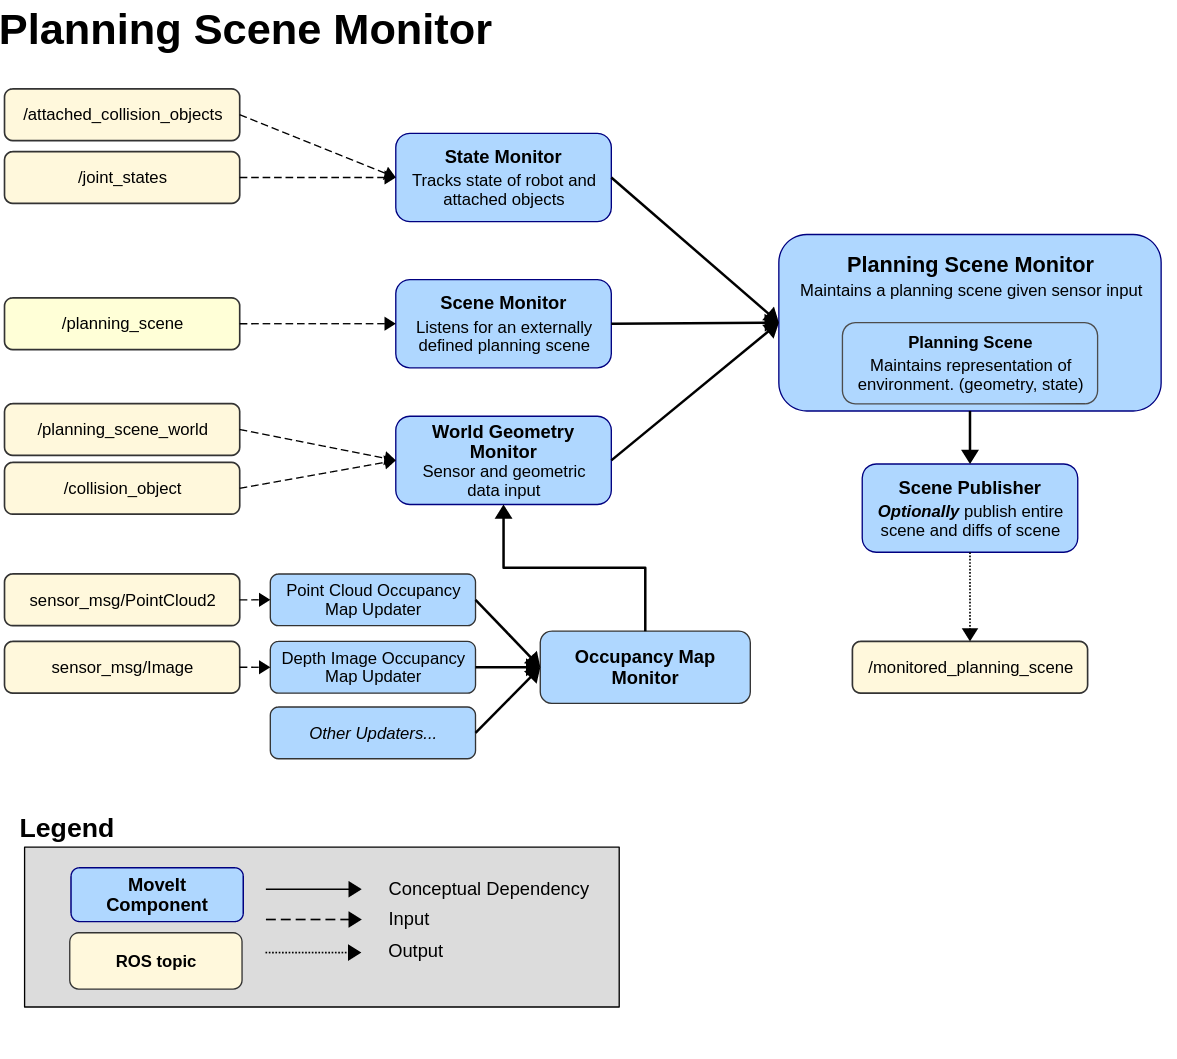
\includegraphics[width=0.8\textwidth]{c4_03.png}
    \caption{Planning Scene and Occupancy Mapping Architecture}
    \label{fig:planninscence}
\end{figure}


\textbf{MoveIt2} is a framework based on ROS2 that provides a set of tools for motion planning, kinematics, control, 
perception, and manipulation. It is a powerful tool for controlling robotic arms and mobile bases, and it can be used to plan and
execute arm trajectories. MoveIt2 is based on the ROS2 middleware and provides a flexible and modular
framework for developing robotic applications.

Figure \ref{fig:moveit2} shows the general \textbf{architecture of MoveIt2}. The MoveIt2 framework consists of several
components, including the Planning Scene, the Planning Pipeline libraries, the Kinematics Solver, the Collision
Checker, the Trajectory Execution Manager, and the Occupancy Mapping tools.
The Planning Scene is a representation of the robot's environment, including the robot's state, the obstacles in the
environment, and the robot's kinematic model. The diagram in Figure \ref{fig:planninscence} shows how the Planning Scene
interacts with the MoveGroup interface, providing the robot's state and kinematic model, and the Occupancy Map,
providing the obstacles in the environment. The Planning Pipeline libraries are used to generate motion plans
for the robot, using the robot's kinematic model and the obstacles in the environment. The Kinematics Solver is
used to compute the robot's joint positions for a given end-effector pose, using the inverse kinematics
computations based on the robot's kinematic model. The Collision Checker is used to check for collisions between
the robot and the obstacles in the environment, using the robot's kinematic model and the obstacles' geometries.
The Trajectory Execution Manager is used to execute the motion plans generated by the Planning Pipeline libraries,
using the robot's joint positions and velocities. The Occupancy Mapping tools are used to generate volumetric 3D 
occupancy maps of the surrounding environment, using depth perception sensors to construct a map
of the obstacles in the environment. 

\begin{figure}[t]
    \centering
    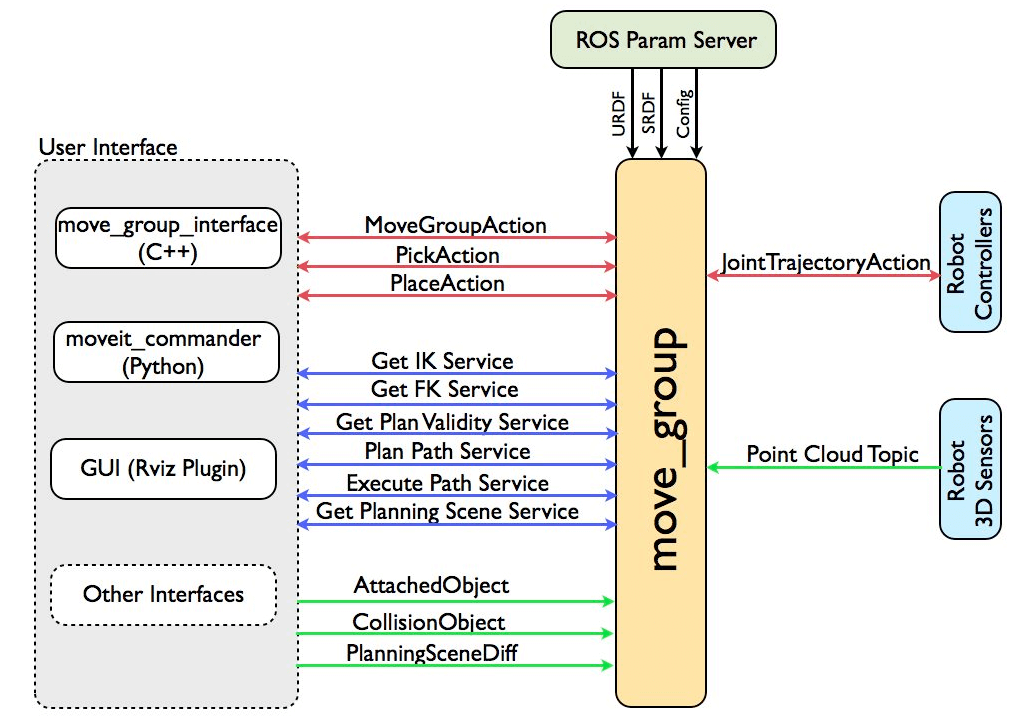
\includegraphics[width=0.8\textwidth]{c4_02.png}
    \caption{MoveGroup Interface}
    \label{fig:move_group}
\end{figure}

MoveIt2 provides the \textit{MoveGroupInterface} class, a high-level interface to the MoveGroup node. The node
provides a set of methods for controlling the robot's motion planning and execution. 
Figure \ref{fig:move_group} shows the architecture and the modules with which it interacts.
The \textit{MoveGroupInterface} provides also methods for interacting with the robot's planning scene, 
including adding and removing obstacles, setting the robot's state, and setting the robot's end-effector pose. 
The \textit{MoveGroupInterface} can be used to plan and execute trajectories for the robot. 
It allows to define and compute joint-space goals, Cartesian-space goals,
and pose goals for the robot's end-effector, which is used to compute the joint space trajectories.

% Add a Figure of the rviz2 interface with moveit2
\begin{figure}[t]
    \centering
    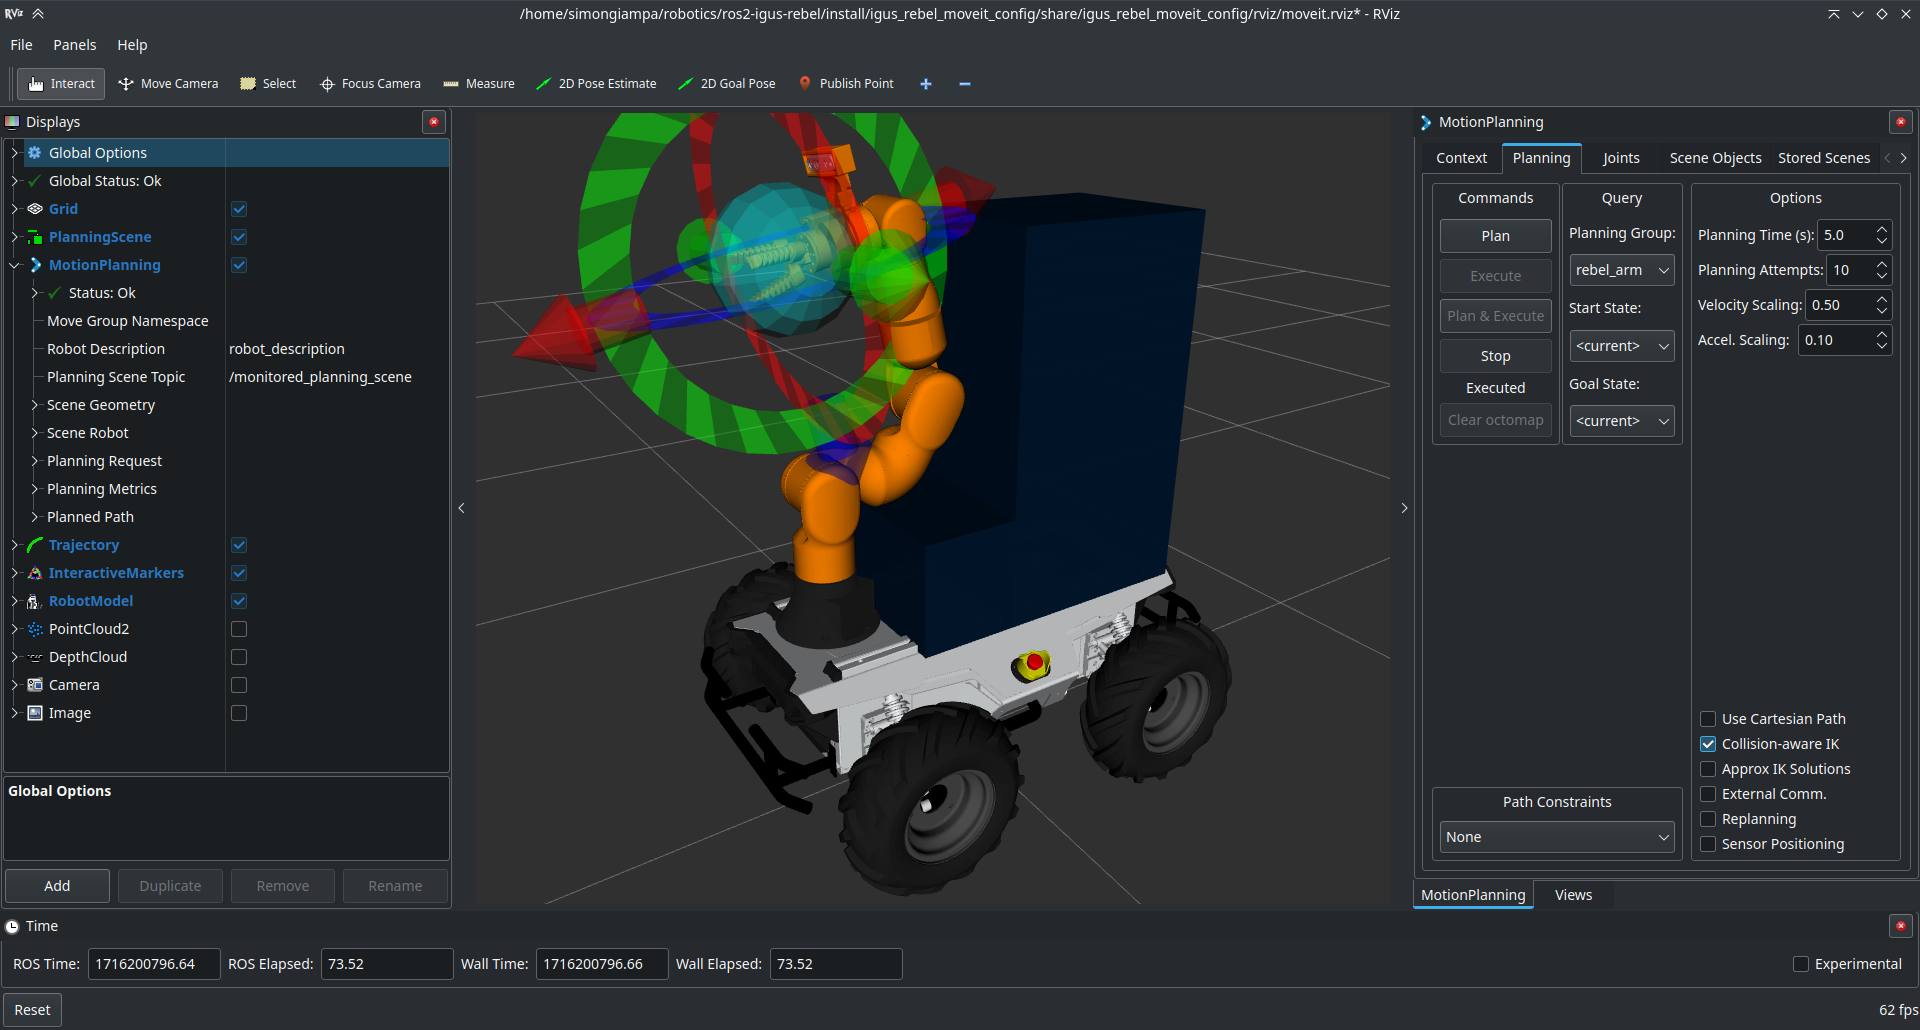
\includegraphics[width=1.0\textwidth]{c4_11.png}
    \caption{RViz2 Interface with MoveIt2 Control Panels and the mobile manipulation robot.}
    \label{fig:rviz2}
\end{figure}


MoveIt2 can be used along with RViz2, a 3D visualization tool for ROS2 to visualize the
robot's motion in both simulated and real environments. RViz2 provides a set of tools for visualizing the robot's
kinematic model, the robot's state, the obstacles in the environment, and the robot's motion plans.
Figure \ref{fig:rviz2} shows a screenshot of the RViz2 interface with the control panels dedicated to the MoveIt2
planning and execution tools. The Figure shows the Igus Rebel cobot mounted on the Scout mobile robot,
with blue collision boxes to prevent the arm from colliding with the sensors mounted on top.
With this interface, it is possible to send joint space goals to the robot
and control it via the underlying hardware interface. There is also an interactive marker that allows the user
to set the robot's end-effector pose by dragging it around in the RViz2 interface.

To ease the development of motion planning and execution for the Igus Rebel arm, a custom ROS2 library was developed.
The library incorporates the \textit{MoveGroupInterface}, providing high-level functions
in C++ that allow to plan and execute different types of motion, as well as computing the end-effector position
and orientation quaternion from sensor input data. This library is based on the MoveGroup lower-level functionalities 
and makes use of different planners to generate a valid motion trajectory given the planning scene, and current and target
joint positions. The planning and execution functions choose the most suitable planner based on the type of motion
to be executed. They also switch planners in the cases of failed motion planning generation.

The planner \textit{Pilz Industrial Motion Planner} is used for linear cartesian trajectories 
since it is more likely to generate feasible plans for this task, compared to the other planners.
The \textit{OMPL} (Open Motion Planning Library) and
\textit{STOMP} (Stochastic Trajectory Optimization) motion planners
are instead used for generating trajectories with joint-space or cartesian-space targets.
The kinematic solver used throughout the project is \textit{KDL} (Kinematics and Dynamics Library), which is a C++ library
that provides a set of tools for computing the forward and inverse kinematics of the robot's kinematic model.
For collision detection, the \textit{FCL} (Flexible Collision Library) is used, which is a C++ library that provides
a set of tools for detecting collisions between the robot and the obstacles in the environment.
Its advantage is the integration with Octomap for 3D collision checking, which is used in the MoveIt2 framework.

One important issue encountered when executing a planned trajectory was the
\textbf{imprecision of the robotic arm's motors' encoders}, which caused the end effector
to not reach the target pose with the desired precision. This problem was partially overcome by adding a function
that artificially compensates for the error in the end effector's position, by adding a small offset 
to the target pose. The formula used for the compensation is based on empirical measurements of the error.
The measurements were taken by commanding the end effector to reach a target pose and then measuring the distance
on the z-axis (vertical axis) between the end effector's final position and the target pose.
The measurements were taken for poses at different heights and distances from the robot's base.
The function is based on the equation 
$z' = z + \frac{1 - z}{25}$, where $z$ is the target position on the z-axis (height) and $z'$ is the corrected target height.
The values used in the formula are expressed in meters.
This function does not provide an accurate compensation for the error, but it is effective in increasing the precision
of the end effector's position.


\section{Robotic Arm Visual Servoing}

The MoveIt2 library provides also a framework for visual servo-ing, a technique used to control the robot's
end-effector pose using visual feedback from a camera. The visual servo-ing framework in MoveIt2 is based on the
\textit{MoveItServo} package, which provides a set of tools for controlling the robot's end-effector pose using
servo-ing algorithms. The servo-ing algorithms are used to compute the robot's joint positions for a given end-effector
pose. A test was set up for the integration of the servo-ing techniques with visual input from the camera.
The test was developed to perform visual servo-ing with the Igus Rebel arm, where the visual input
is provided by the estimation of an ArUco marker's pose in the camera's field of view, and the servo-ing algorithm
is used to track the marker's pose and move the arm's end-effector as close as possible orthogonally to the marker's pose.

The servo-ing algorithms provided by MoveIt2 enable \textbf{real-time control and teleoperation} of the robot arm's
end-effector pose. The teleoperation allows the user to control the robot's end-effector pose using a joystick controller.
The real-time control consists of controlling the robot's end-effector pose using camera visual feedback
in real-time without pre-computing the joint trajectories. Realtime control is useful for controlling the robot's
end-effector pose in dynamic environments, where the obstacles are moving and the robot needs to adapt to the changes
in the environment.

\begin{figure}[t]
    \centering
    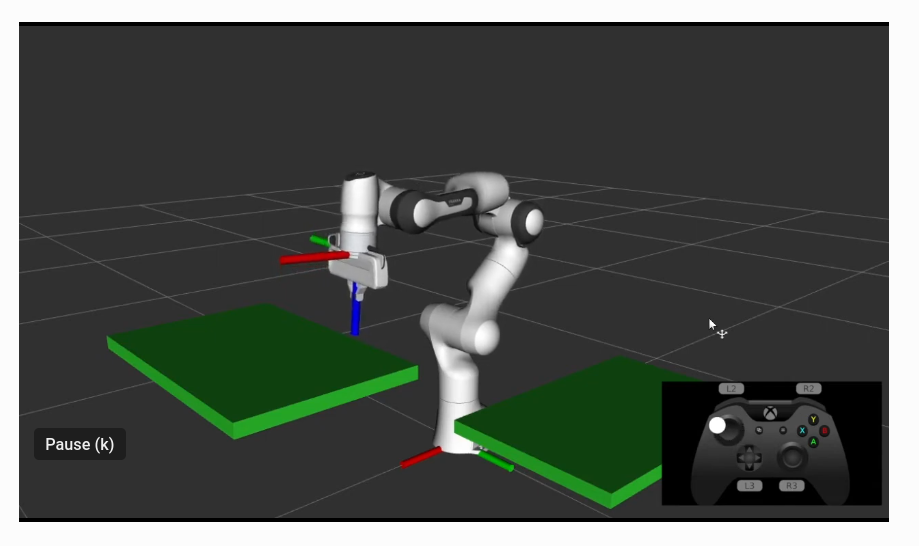
\includegraphics[width=0.8\textwidth]{c4_05.png}
    \caption{Teleoperation with a joystick controller in RViz2 with the Franka Emika Panda}
    \label{fig:teleop}
\end{figure}

Visual servo-ing functionality was implemented and achieved partial success, operating reliably with input 
Cartesian poses near the arm's initial configuration. The servo-ing algorithm's reliance on accurate initial
end-effector pose estimates presented challenges in achieving convergence to desired poses under varying conditions.
The servo-ing algorithm was tested with dynamically generated input cartesian poses, and the algorithm performance
evaluation is based on the arm's ability to reach the desired poses consistently. 
\textit{PlotJuggler} is the software used to plot the trajectory of each joint in time, which is necessary 
for monitoring and measuring the degree of the oscillations and overshooting of the arm's joints during the servo-ing process
until convergence to the input pose is achieved.

Open-loop control tests highlighted the algorithm's sensitivity to joint position errors, hindering its ability
to reach desired poses consistently. While switching to closed-loop mode offered the potential for error compensation, 
it requires a PID controller to operate. Since the PID controller's performance was hampered by the need for 
further gain tuning to mitigate strong oscillations, the tests were conducted only in the simulated environment,
where a PID controller was easier to tune. The effort required to identify the optimal gains for the PID controller
was beyond the gain obtained using this approach.
Despite these challenges, the implemented visual servo-ing package remains available within the repository as a foundation
for future development. However, due to the limitations encountered in achieving stable and reliable performance,
it was not incorporated into the final mobile manipulation system implementation.

\section{Collision Avoidance with Octomap}

The MoveIt2 library provides a framework for collision avoidance using \textbf{Octomap}, a library for
generating volumetric 3D occupancy maps of the surrounding environment \cite{hornung13octomap}.
Octomap is a 3D probabilistic occupancy grid representation of the robot's environment. It divides the space into voxels
(3D cubes) and assigns probabilities to each voxel, indicating whether it's occupied or free.
MoveIt2 integrates data from depth sensors, such as a depth camera or a LiDAR, to update the Octomap in real time.
Figure \ref{fig:octomap} shows the integration of Octomap inside MoveIt2, where the voxels defining the occupancy
mapping are inside the Planning Scene. The motion planning algorithms can use the voxels to plan a trajectory
that avoids them.

MoveIt2's collision checker uses Octomap to efficiently check for collisions between the robot's planned trajectory
and the environment. By checking if the voxels along the path are occupied, it can determine if the robot will collide 
with any obstacles. The probabilistic nature of Octomap helps deal with sensor noise and uncertainty. 
If a voxel has a high probability of being occupied, it's treated as an obstacle.

MoveIt2's motion planners, such as \textit{OMPL} (Open Motion Planning Library), use Octomap
to generate collision-free paths. The planners avoid occupied voxels to ensure the robot's motion doesn't lead to collisions.
If the environment changes during execution (e.g., an obstacle moves), MoveIt2 can use the updated Octomap 
to quickly replan a new collision-free path, allowing for dynamic obstacle avoidance.
This allows for a dynamic representation of the environment, even if obstacles move.

% Add a screenshot of the Octomap in RViz2
\begin{figure}[t]
    \centering
    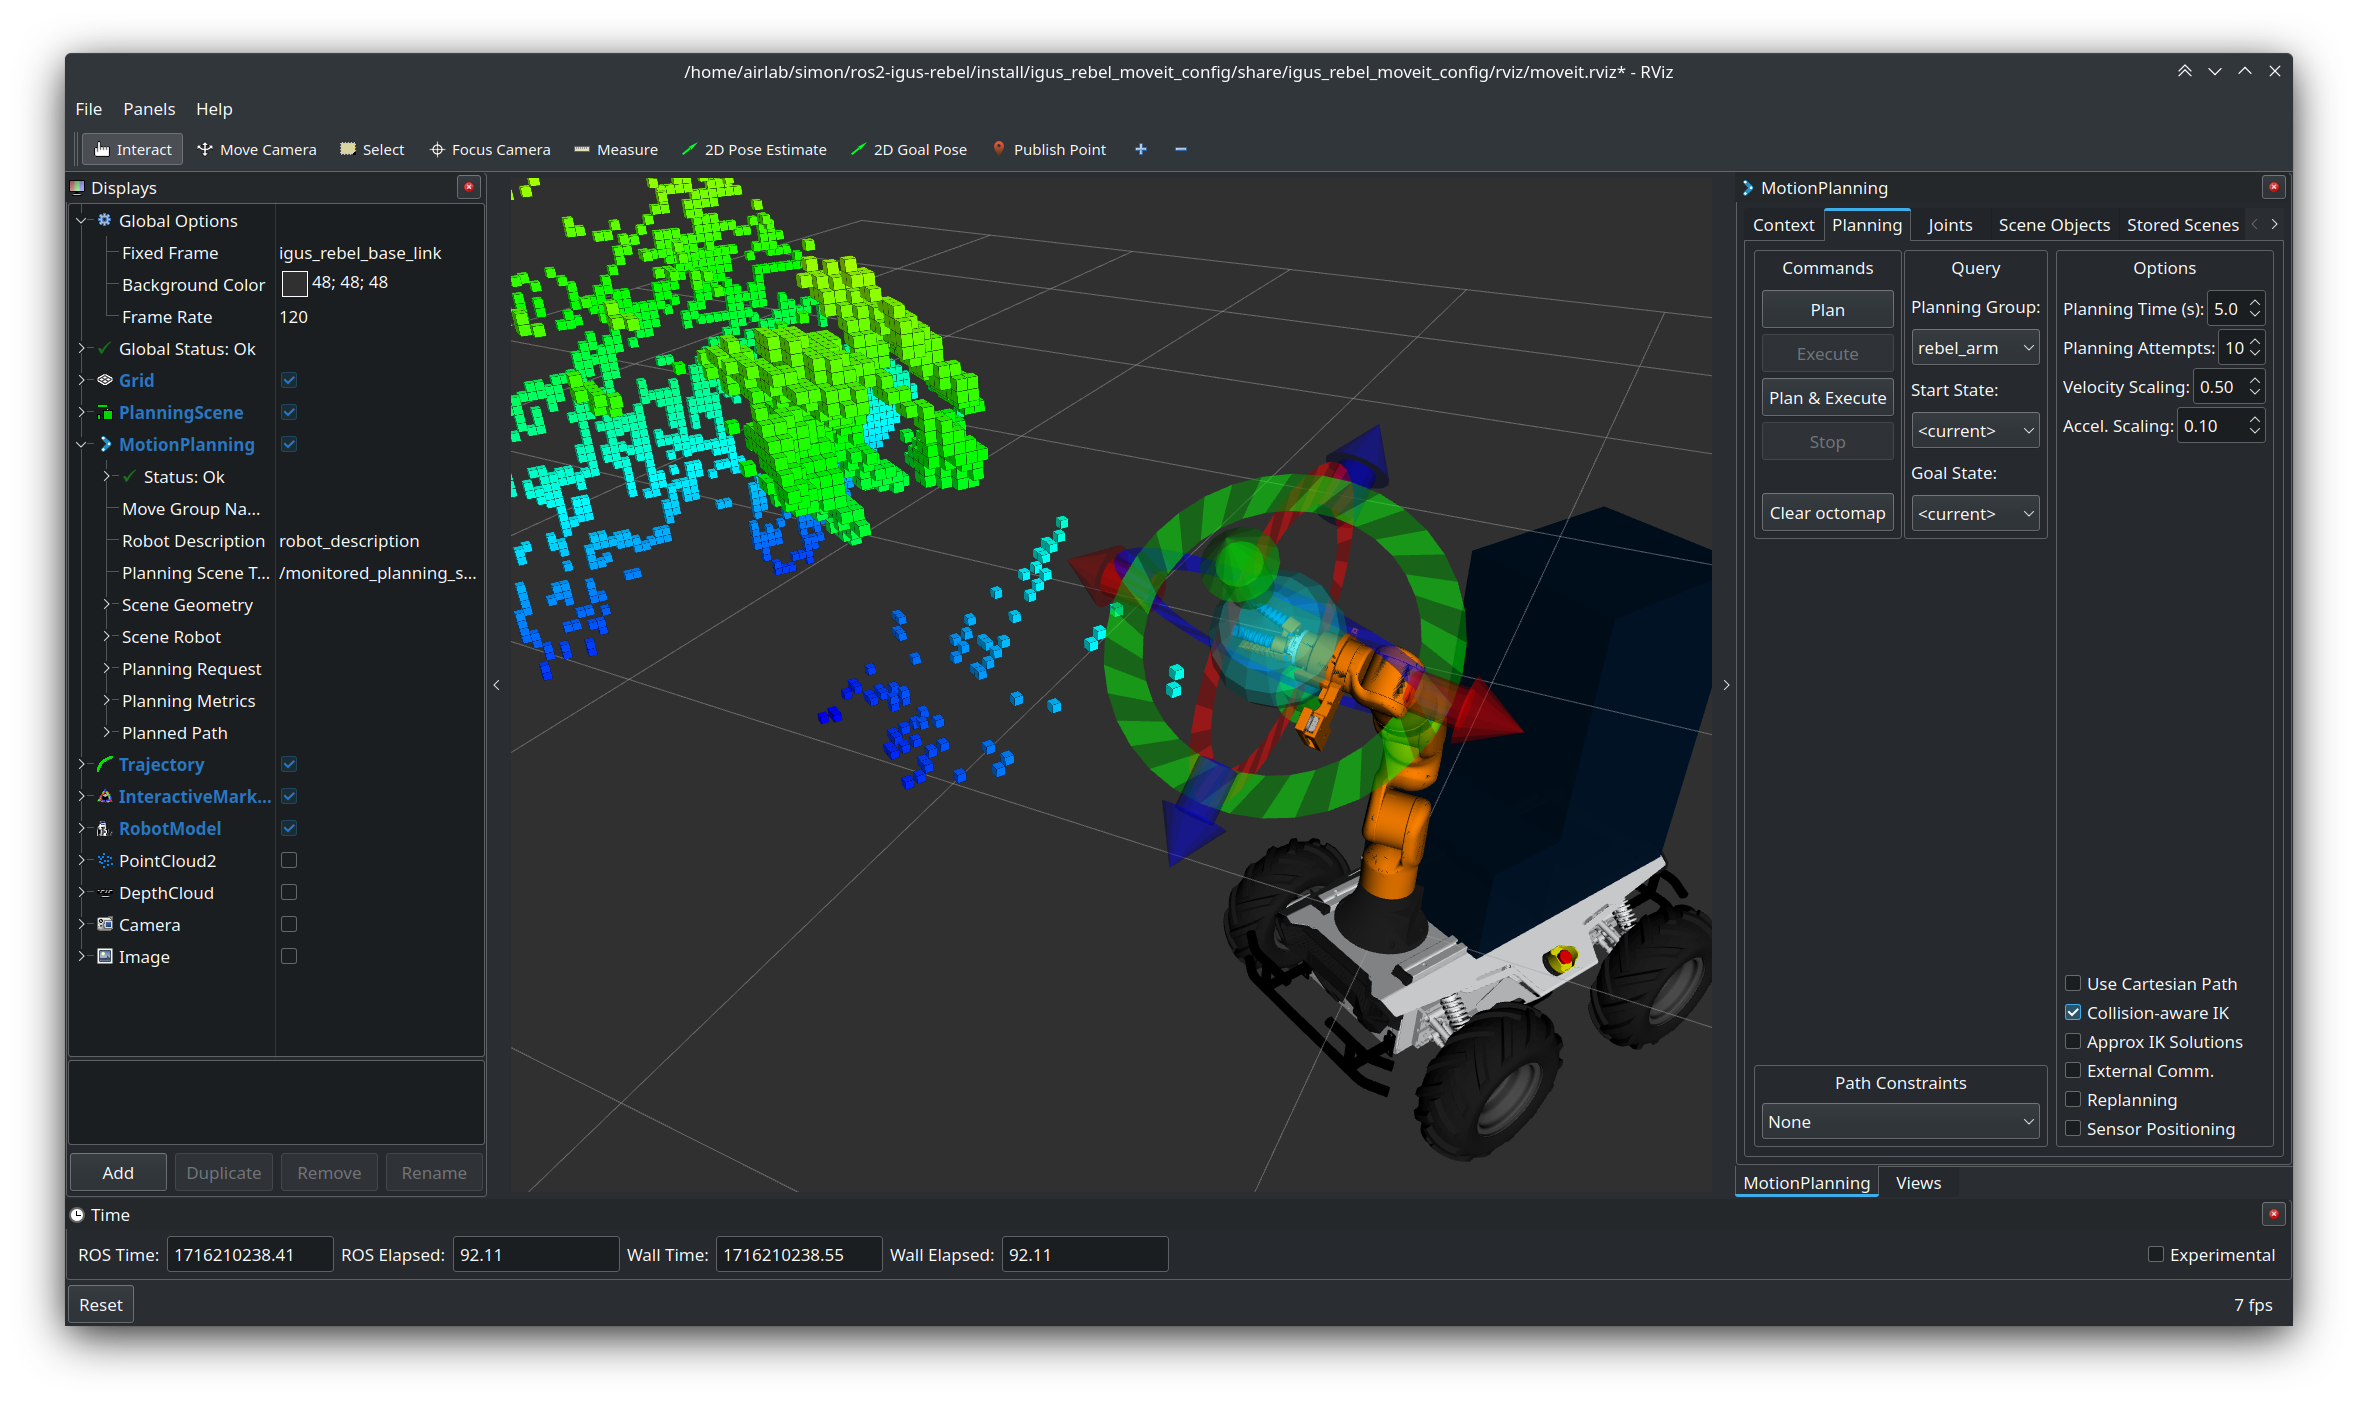
\includegraphics[width=1.0\textwidth]{c4_15.png}
    \caption{Mobile robot using the depth camera to construct the Octomap with the obstacles nearby}
    \label{fig:octomap}
\end{figure}

However, the reality is far from the ideal scenario. The Octomap library is not yet fully integrated with MoveIt2,
resulting in a \textbf{poorly optimized} Octomap probabilistic representation of the environment.
In fact, the library tracks the free space as well as the occupied space, meaning that the entire workspace volume
of Octomap is indexed within the data structure for volumetric representation, resulting in a memory and computationally
intensive update process. This results in low-frequency updates of the voxels. Octomap
library for ROS2 is a yet incomplete porting of its ROS1 counterpart.

The ability to update the Octomap in realtime when part of the environment changes is still a missing feature.
In the current version of the software, Octomap will only update a few voxels around the
part of the environment that changed, without fully removing the voxels corresponding to the obstacle that moved
and that is not present in the scene anymore. This leads to \textbf{false positives in the collision checking}, which
prevents the robot from executing the planned trajectory. This feature is critical for dynamic obstacle avoidance
because the robot needs to avoid the voxels corresponding to the obstacles and touch the voxels corresponding
to the object that the end effector needs to grasp. This means that not only does the robot need to avoid the obstacles
but also understand which voxels the robot arm can collide with.
The Octomap Library is still under development, and it is expected to be correctly integrated with MoveIt2 in the future.

\section{Soft Gripper Pneumatic Pump Actuation}

The soft gripper is actuated using a ROS2-control interface that acts as a hardware interface to the Arduino UNO
microcontroller that controls the pneumatic pump. The hardware interface works by providing a ROS2 service server that 
listens for commands to open or close the gripper and sends the corresponding commands to the Arduino UNO microcontroller
via serial communication. 
Serial communication uses the UART protocol to send and receive plain text messages.
The serial data transfer is done using the \textit{thermios} library, which is a POSIX-compliant library for serial
communication in Linux, supporting the C language.

The \textbf{Arduino UNO microcontroller} is programmed to control the pneumatic pump by changing
the state of the relays connected to its digital pins. The Arduino UNO listens in the serial port for string commands
that it interprets as the pins to be set high or low, to open or close the gripper. The pneumatic pump is connected
to the Arduino UNO via a relay module with 4 relays, one for each digital pin of the pump. Two of which
are the VCC and GND pins, and the other two are the GRIP and RELEASE pins. The GRIP pin is used to close the gripper,
while the RELEASE pin is used to open the gripper.


\section{Ignition Gazebo Simulation Environment}

Ignition Gazebo is a useful open-source simulation environment for robotics and autonomous systems.
It provides a realistic and customizable 3D environment for testing and developing robotic algorithms and applications.
\textbf{Ignition Gazebo} is the simulation environment of choice for the project,
as it proved to be very useful in testing the mobile robot base in simulated environments before deploying the algorithms
on the real robot. Simulating the robot in a virtual environment allows for testing the algorithms in 
a controlled and repeatable environment, without the risk of damaging the real robot or the laboratory environment.
The simulations were essential for the development of the software and the navigation algorithms, 
as they allowed for testing
the robot's behavior in different scenarios and environments. It allowed me to tune Nav2's parameters
thoroughly and ensure the robot would avoid obstacles and navigate safely.

% add a screenshot of the simulation environment in Ignition Gazebo
\begin{figure}[t]
    \centering
    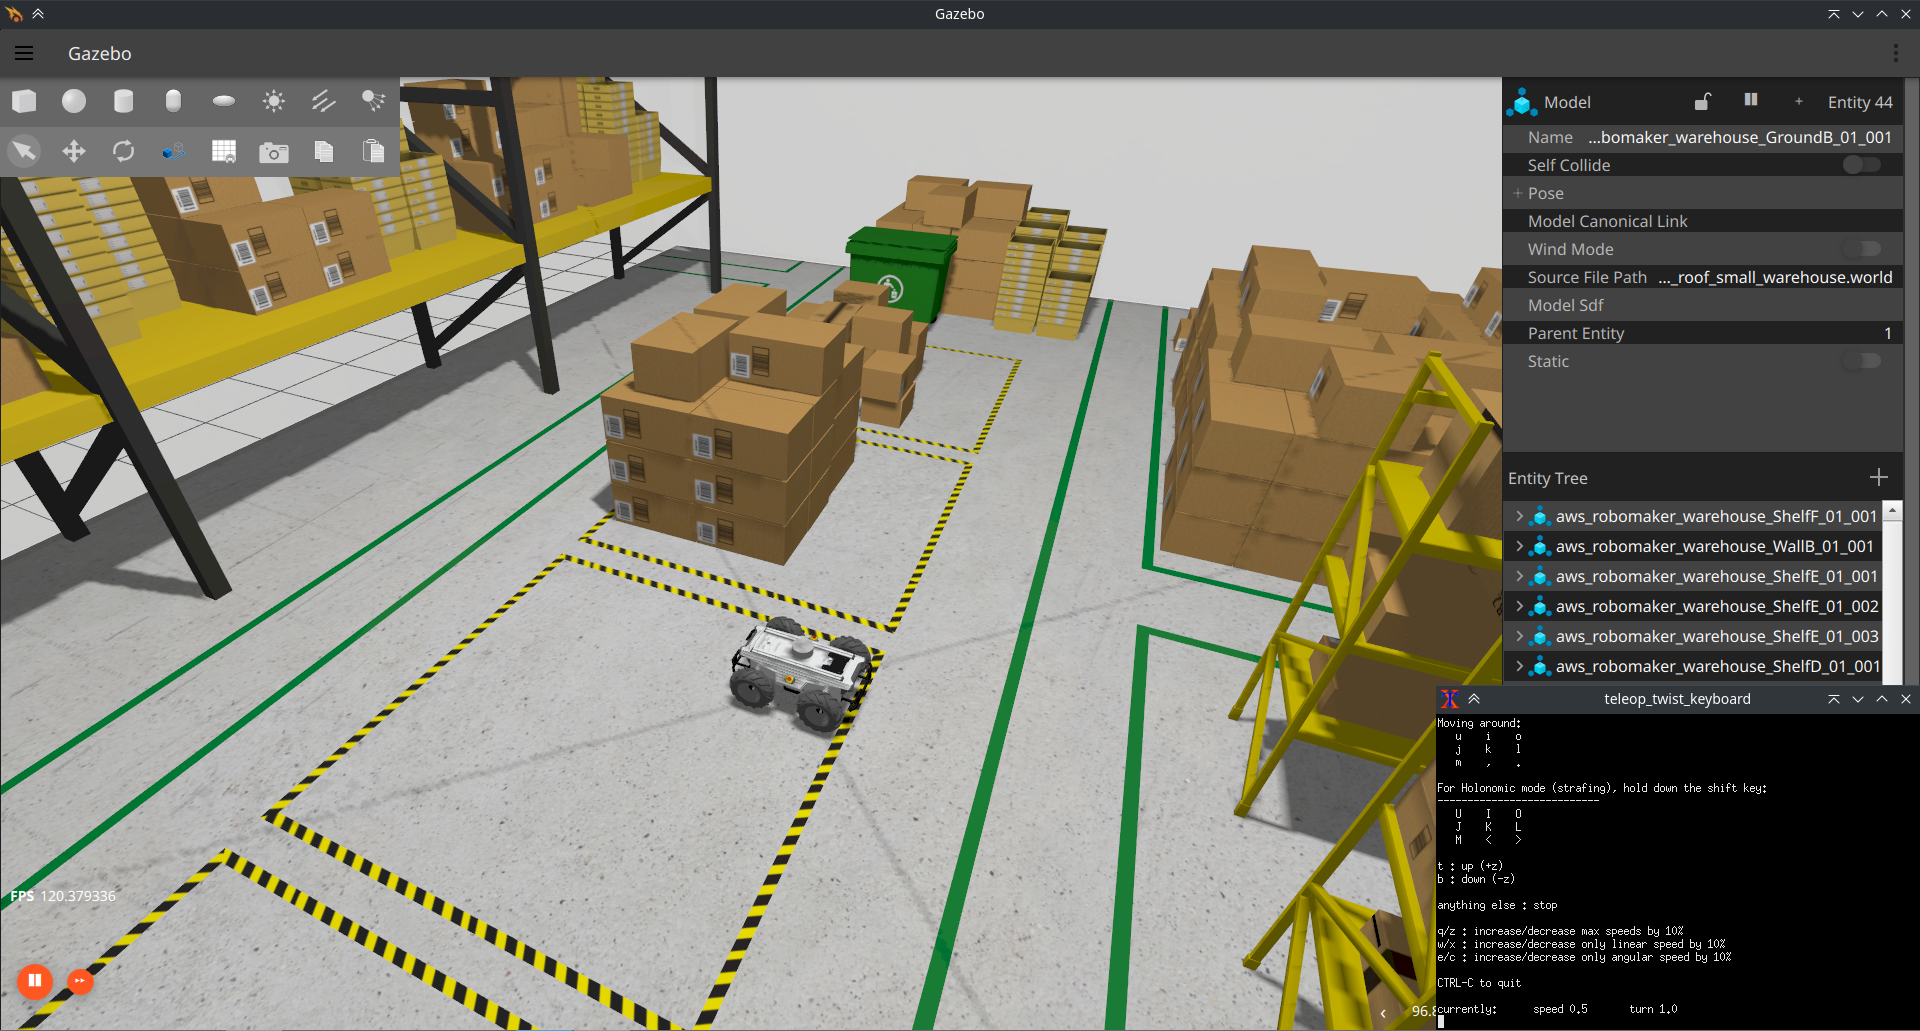
\includegraphics[width=1.0\textwidth]{c4_12.png}
    \caption{Ignition Gazebo Simulation Environment}
    \label{fig:ignition}
\end{figure}

% Add the created map of the warehouse
\begin{figure}[t]
    \centering
    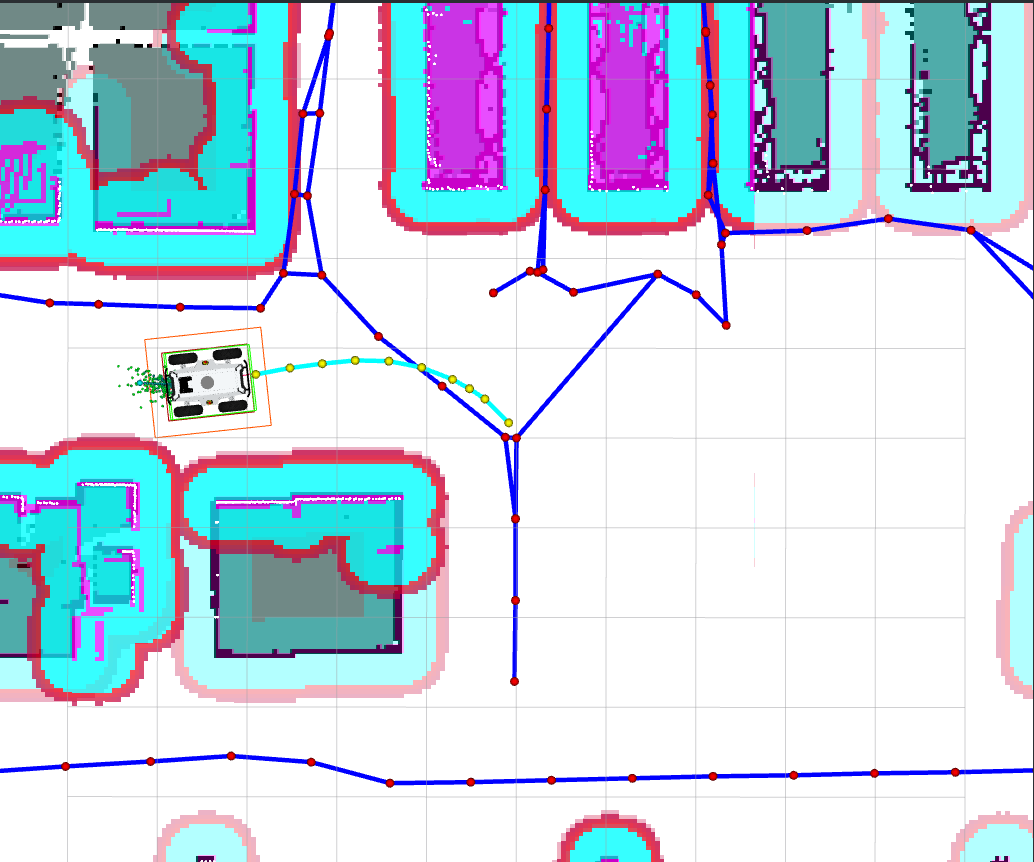
\includegraphics[width=1.0\textwidth]{c4_14.png}
    \caption{Mobile robot navigating in the simulated warehouse environment}
    \label{fig:warehousenav2}
\end{figure}

The simulated environment in Ignition Gazebo used for the project is a \textbf{warehouse}
with various obstacles such as walls, shelves, and boxes, which the robot had to navigate around to reach its goal.
Figure \ref{fig:ignition} shows a screenshot of the simulated warehouse environment in Ignition Gazebo.
The warehouse environment was designed to be challenging
for the robot, with narrow passages and tight spaces, to test the robot's ability to navigate in complex environments.
Ignition Gazebo also provides the possibility to add dynamic obstacles, i.e. objects not present in the map
already loaded in the simulation environment. This feature was useful for testing the robot's dynamic obstacle avoidance
algorithm, which allows the robot to navigate safely in environments with unknown obstacles.

The simulation also includes the sensors mounted on the robot, such as a 2D LiDAR and a 3D LiDAR sensor, which were used
for perception and obstacle avoidance. The localization algorithms, such as AMCL and SLAM Toolbox,
were tested using the simulated odometry data created by the robot's wheels' motion in the simulated environment. Figure 
\ref{fig:warehousenav2} shows the simulated mobile robot navigating in the warehouse environment
while avoiding the boxes and shelves in its path.

\section{Autonomous Navigation with NAV2}
\label{sec:nav2}

Nav2 is a powerful open-source software framework used for autonomous navigation within the ROS2 ecosystem
\cite{macenski2020nav2}.
It provides a comprehensive set of tools and algorithms for enabling robots to navigate complex environments intelligently.
With Nav2, robots can perceive their surroundings, localize themselves, plan optimal paths, and execute 
those paths while avoiding obstacles. Its modular architecture allows for customization and integration with various sensors,
such as LiDAR and cameras, making it adaptable to different robot platforms and use cases. 
Nav2's flexibility and robust features make it a popular choice for both research and industrial applications 
in fields like robotics and autonomous vehicles
\cite{macenski2023survey}.

Nav2's \textbf{modular architecture} enables the seamless integration of various plugins that contribute
to its robust autonomous navigation capabilities. Costmap plugins, such as static and obstacle layers,
create a real-time representation of the robot's environment, highlighting obstacles and free space. 
Collision monitors continuously assess the robot's planned path against this costmap ensuring safe navigation.
Localizers, like AMCL, estimate the robot's position within the environment, while mappers like SLAM create and update maps
of the surroundings. Planners, such as global planners (e.g., Hybrid A*) and local planners (e.g., DWB),
work in tandem to generate collision-free paths for the robot to follow, enabling efficient and fast navigation. 
Additionally, plugins like controllers and recovery behaviors further enhance Nav2's ability to handle unexpected
scenarios and ensure the robot reaches its goal.

Given these premises and features, Nav2 was selected as the primary navigation system for the mobile manipulator robot.
The Nav2 framework is used to plan and execute trajectories for the mobile base, using the robot's
LiDAR sensor to perceive the environment and avoid obstacles. The framework operates within a ROS2 
composable node architecture, which allows for the integration of various plugins and algorithms to achieve
efficient intra-process communication and data sharing between the various components and threads of the multiple plugins.
The parameters for Nav2 were configured specifically to work with the AgileX Scout robot, using the SLAM Toolbox algorithm
for mapping and localization. Figure \ref{fig:nav2_hallway} and Figure \ref{fig:nav2_airlab} show the autonomous
navigation of the robot in the hallways and AIRlab in building 7 of Politecnico di Milano, respectively.

% Add screenshots of the map and costmap in RViz2
\begin{figure}[t]
    \centering
    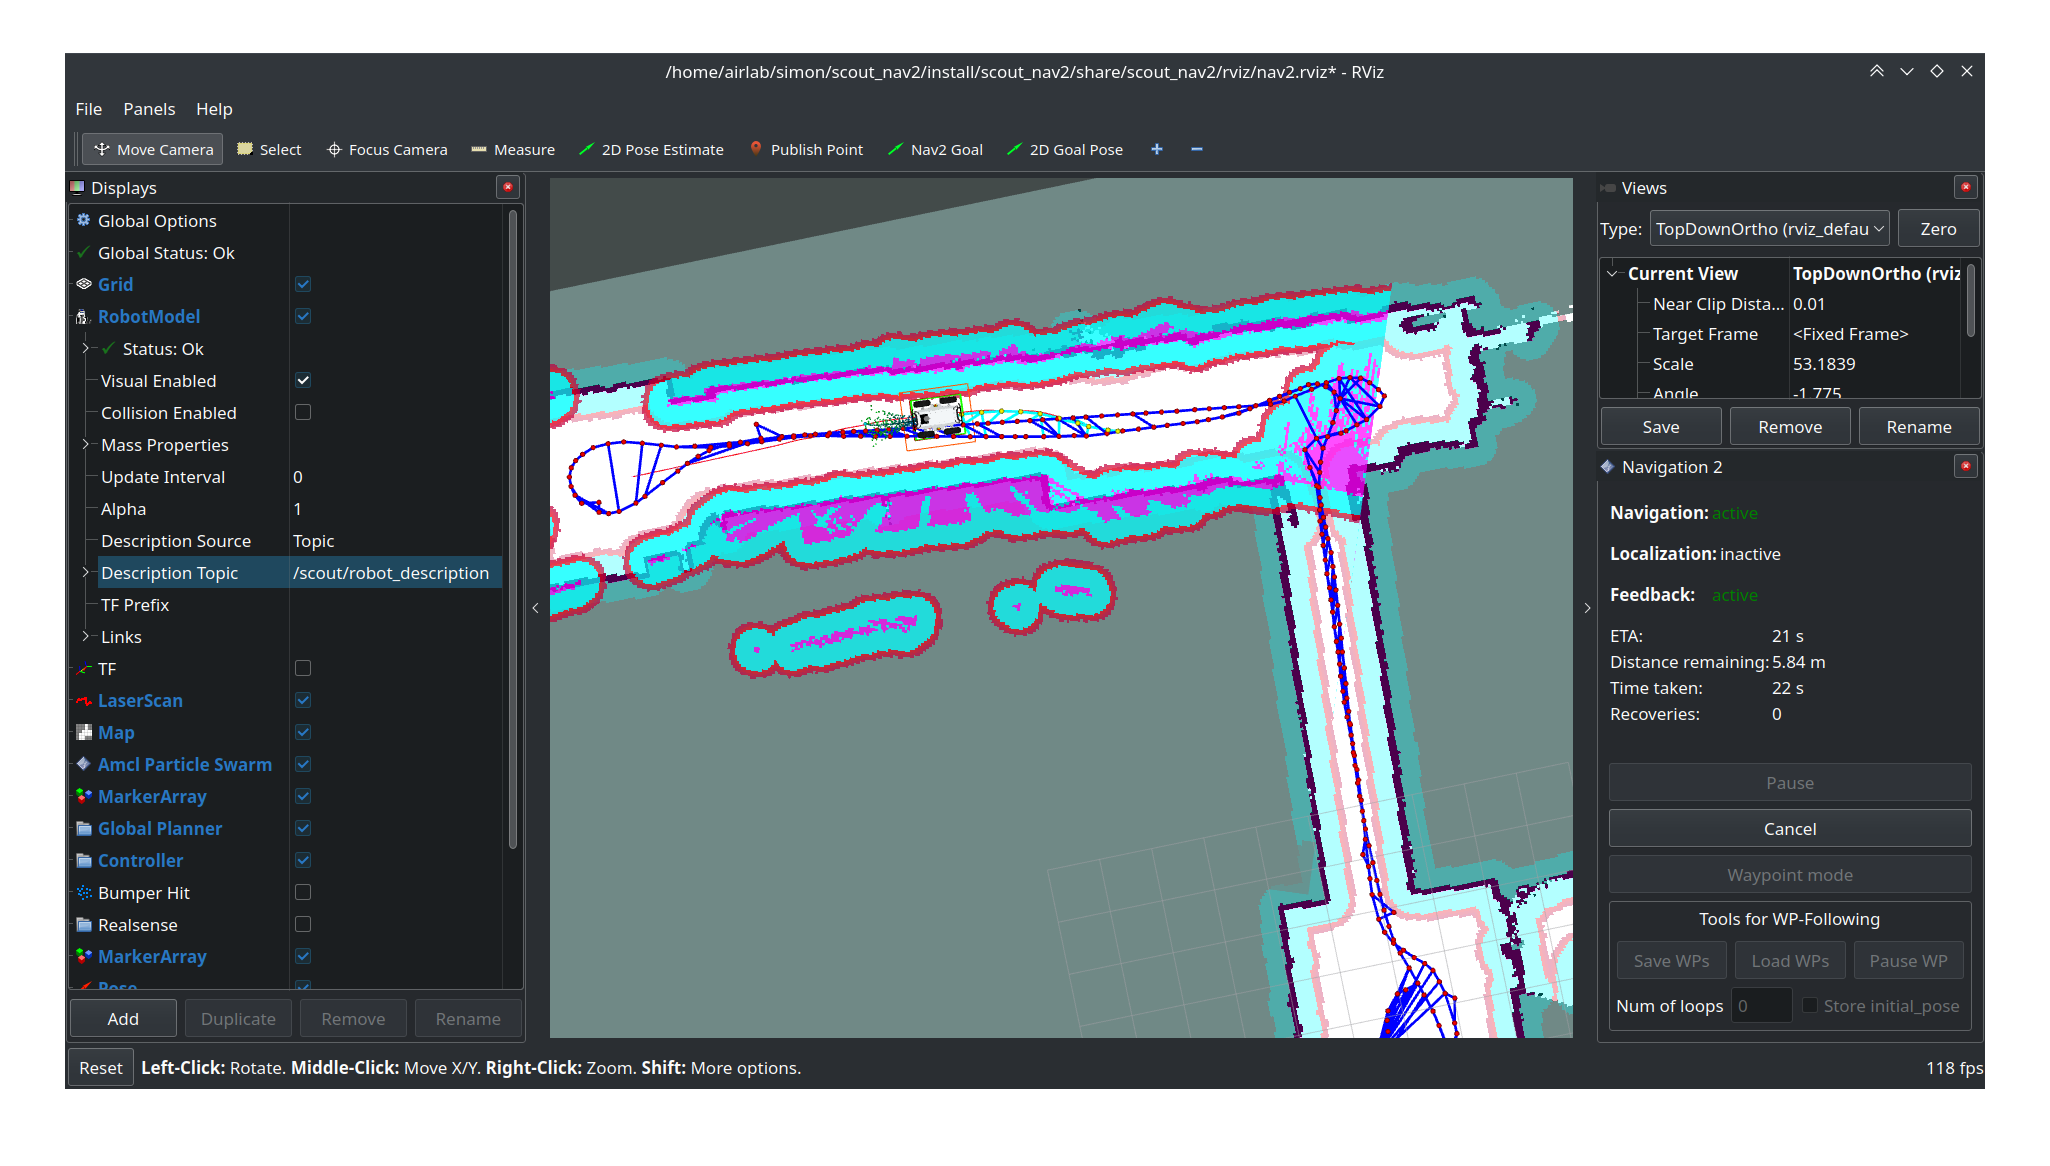
\includegraphics[width=1.0\textwidth]{c4_20.png}
    \caption{Autonomous Navigation with Nav2 in the hallways of building 7 of Politecnico di Milano}
    \label{fig:nav2_hallway}
\end{figure}

\begin{figure}[t]
    \centering
    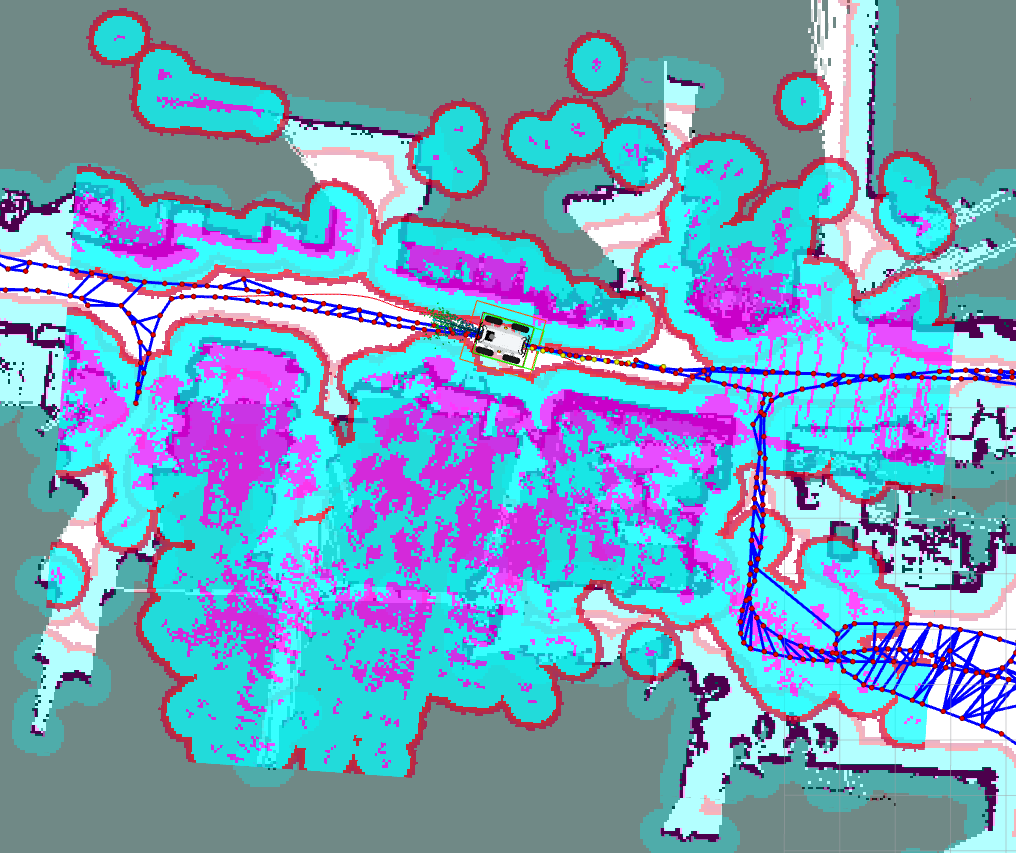
\includegraphics[width=1.0\textwidth]{c4_22.png}
    \caption{Autonomous Navigation in cluttered and dynamic environment with moving obstacles (AIRlab)}
    \label{fig:nav2_airlab}
\end{figure}

\subsection{Nav2 Parameters Tuning}

Finding the right parameters for the Nav2 framework required tuning hundreds of parameters to achieve optimal performance.
The parameters to be set are related to all the plugins that are included within Nav2. 
Many tests in different and complex environments were performed to find the best parameters
suitable for the AgileX Scout robot. The parameters were tuned in both simulated
and real environments, to ensure that the robot can navigate safely and efficiently in different scenarios.

\textbf{Localization Algorithms}:
The algorithms under test were Adaptive Monte Carlo Localization (AMCL) and SLAM Toolbox.
The results of the tests showed that AMCL has a worse performance for in-place rotations.
SLAM Toolbox algorithm has better performance and improved reliability in terms of localization accuracy,
even in changing environments with dynamic obstacles. Therefore it was selected as the primary localization algorithm.
The pose graph generated by the SLAM Toolbox algorithm
is displayed in the maps, as shown in Figure \ref{fig:nav2_hallway} and Figure \ref{fig:nav2_airlab}, where the
blue lines represent the pose graph created during map creation, and the cyan lines represent the robot's
the path traversed during navigation, estimated by the algorithm and connected to one of the nodes in the pose graph.

\textbf{Global Planner}:
SMAC planners \cite{macenski2024smac} are used as global path planners, in particular the Hybrid A* global planner.
Hybrid A* performs well in generating optimal paths for the robot to follow, 
even in cases where an unknown obstacle appears in the environment. The Hybrid A*
global planner uses an A* search algorithm to generate optimal paths for the robot to follow, which allows the robot
to compute efficient paths and adjust quickly to changes in the environment. The Hybrid A* global planner is based on
the motion generation algorithm, which generates kinematically feasible paths for the robot to follow, and the path selection
algorithm, which selects the best path from the sample paths based on the cost function.
The motion generation algorithms available are the \textit{Dubin} and \textit{Reeds-Shepp} algorithms, which both generate
kinematically feasible motion trajectories. The Reeds-Shepp algorithm enables
the generation of paths also in the reverse direction, which is useful for navigating in reverse, especially for
a skid-steering drive robot such as the Scout. However, probably due to some bugs within Ignition Gazebo,
the Reeds-Shepp algorithm works only with the real Scout robot, and not with the simulated one in the Gazebo environment.

\textbf{Local Planner (Controller)}:
Two local planners were tested: DWB and MPPI.
The MPPI (Model Predictive Path Integral Controller) \cite{mppicontroller}
local planner uses a \textbf{model predictive control approach}
to generate collision-free paths for the robot to follow, which allows the robot to navigate efficiently in complex
environments with tight spaces and obstacles. The MPPI local planner also provides better performance in terms of
trajectory tracking and collision avoidance, compared to the DWB local planner. 
The DWB local planner uses a dynamic window approach to generate
collision-free paths for the robot to follow, which can be less effective in tight spaces and complex environments.
The sampled trajectories of the local planner are visualized in Figure \ref{fig:nav2_hallway} and Figure \ref{fig:nav2_airlab},
in front of the robot's footprint, showing the robot's sampled trajectories to follow the global path.

\textbf{Recovery Behaviors}:
The default recovery behaviors provided by the recovery behavior tree plugin of Nav2
perform well in recovering the robot from unexpected scenarios, such as getting stuck or colliding with obstacles.
However, in the most difficult scenarios, using the default recovery behaviors, the robot was not able to recover quickly
from the situations where it was stuck near an obstacle, and it was unable to move for long periods.
Therefore some slight modifications to the default recovery behaviors were applied to improve the robot's response
in recovering from the scenarios where the robot would be unable to move, making it faster to recover and continue
navigating towards the goal. The modified recovery behaviors
include a combination of back-up and rotate behaviors, which allow the robot to back up and rotate in place to position
itself in a different configuration, enabling it to generate a new path and continue navigating towards the goal.

\textbf{Local Costmap}:
The local costmap plugin is used to generate a local costmap of the robot's surroundings, highlighting obstacles
and free space. The local costmap plugin uses the robot's LiDAR sensor to perceive the environment and update the costmap
in realtime. The local costmap plugin is used by the local planner to generate collision-free paths for the robot
to follow. The local costmap includes the unknown obstacles in the environment, which are represented as pink areas
in the costmap, as shown in Figure \ref{fig:nav2_airlab}. The unknown obstacles are detected by the LiDAR sensor
and updated in the costmap, allowing the robot to avoid collisions with objects not present on the map.
The local costmap can be configured with these plugins:

\begin{itemize}
    \item \textbf{Inflation Layer}: The inflation layer is used to inflate the obstacles in the costmap, creating a buffer
    around the obstacles to ensure that the robot avoids collisions.
    \item \textbf{Obstacle Layer}: The obstacle layer is used to update the costmap with the obstacles detected by
    the 2D LiDAR sensor, highlighting the obstacles in the costmap. This layer was eventually substituted with the voxel layer,
    thanks to the more effective 3D LiDAR sensor perception.
    \item \textbf{Static Layer}: The static layer is used to update the costmap with the static obstacles in the map
    \item \textbf{Voxel Layer}: The voxel layer is used to update the costmap with the voxelized obstacles in the map,
    using the 3D LiDAR sensor to perceive the environment and update the costmap in realtime.
\end{itemize}

\textbf{Global Costmap}:
The global costmap plugin is used to generate a costmap of the entire map that the robot is navigating in, highlighting
the static obstacles and free space. The global costmap plugin is used by the global planner to generate optimal paths
for the robot to follow. The global costmap is configured to use only the static layer inflated by the inflation layer,
to ensure that the robot avoids collisions with the obstacles already present in the map.
The global costmap is represented in Figure \ref{fig:nav2_hallway} as the blue and red areas, where the blue areas are the 
\textit{lethal} space (i.e. must be avoided) and the red areas are the inflated obstacle areas with high cost.

\textbf{Collision Monitor}:
The collision monitor plugin is used to continuously assess the robot's planned path against the costmap, ensuring
that the robot navigates safely and avoids collisions with obstacles. The collision monitor plugin is used by
Nav2 to ensure that the robot avoids the obstacles in the costmap, such that they do not overlap with the robot's
footprint and locally planned path.

\textbf{Mapping Algorithm}:
The algorithm of choice for mapping is \textit{SLAM Toolbox}, a 2D SLAM algorithm
that uses the robot's LiDAR sensor to create a 2D map of the environment \cite{Macenski2021slamtoolbox}.
SLAM Toolbox creates a 2D map of the environment used by the global planner to generate optimal paths for the robot to follow.
The SLAM Toolbox proved to be effective in creating accurate 2D maps of the environment, even in dynamic environments
with moving obstacles. This algorithm demonstrated good performance in terms of mapping accuracy and reliability,
both in the simulated and real environments.

\textbf{Velocity Smoother}:
The velocity smoother plugin is used to smooth the robot's velocity commands, ensuring that the robot moves smoothly
and efficiently in the environment. The velocity smoother plugin is used by the local planner to obtain
trajectories with a smooth velocity profile, computed from the initial optimal paths, which allows
the robot to navigate efficiently and avoid jerky movements. The velocity smoother is configured also to avoid
unnecessary stops and starts, which can wear out the robot's transmission gears and reduce the robot's battery life.

\textbf{Spatio-Temporal Voxel Costmap Layer} \cite{macenski2020stvl}:
The dynamic obstacle avoidance algorithm is a critical component of Nav2, as it allows the robot to navigate
safely in dynamic environments with moving obstacles. The dynamic obstacle avoidance algorithm uses the robot's LiDAR sensor
to perceive the environment and detect the moving obstacles in realtime. Dynamic obstacles update the local costmap
following different plugins, such as the voxel layer, which is used to update the costmap with the voxelized obstacles
in the environment. The voxel layer uses the 3D LiDAR sensor to perceive the environment and update the costmap.
However, one of the shortcomings of the voxel layer is that it doesn't remove old voxels that correspond to obstacles
that are no longer present in the environment. This leads to false positives in the collision checking, which prevents
the robot from executing the planned trajectory, especially in highly dynamic environments with fast-moving obstacles.
The spatio-temporal voxel costmap layer (STVL) is an open-source plugin that addresses this issue by updating the costmap
efficiently and accurately. It replaces the traditional voxel grid approach with a \textbf{sparse voxel grid} implemented
using OpenVDB, a \textbf{high-performance C++ library}. This allows STVL to handle large, dynamic environments with ease,
such as the one shown in Figure \ref{fig:stvl}, 
reducing computational overhead. By leveraging temporal information and applying a voxel grid filter to sensor data,
STVL can better handle noisy and dense sensor readings, especially in proximity to objects. 
This results in smoother, more reliable navigation and improved robot performance in continuously evolving scenarios.
STVL's adaptability, efficiency, and ability to integrate with various sensor types made it the ideal substitute
for the voxel layer in Nav2. Figure \ref{fig:nav2_airlab} shows the effectiveness of the STVL in a dynamic
and cluttered environment, such as the AIRLab, where the robot is navigating despite many unknown obstacles 
and moving objects in a tight space.

\begin{figure}[t]
    \centering
    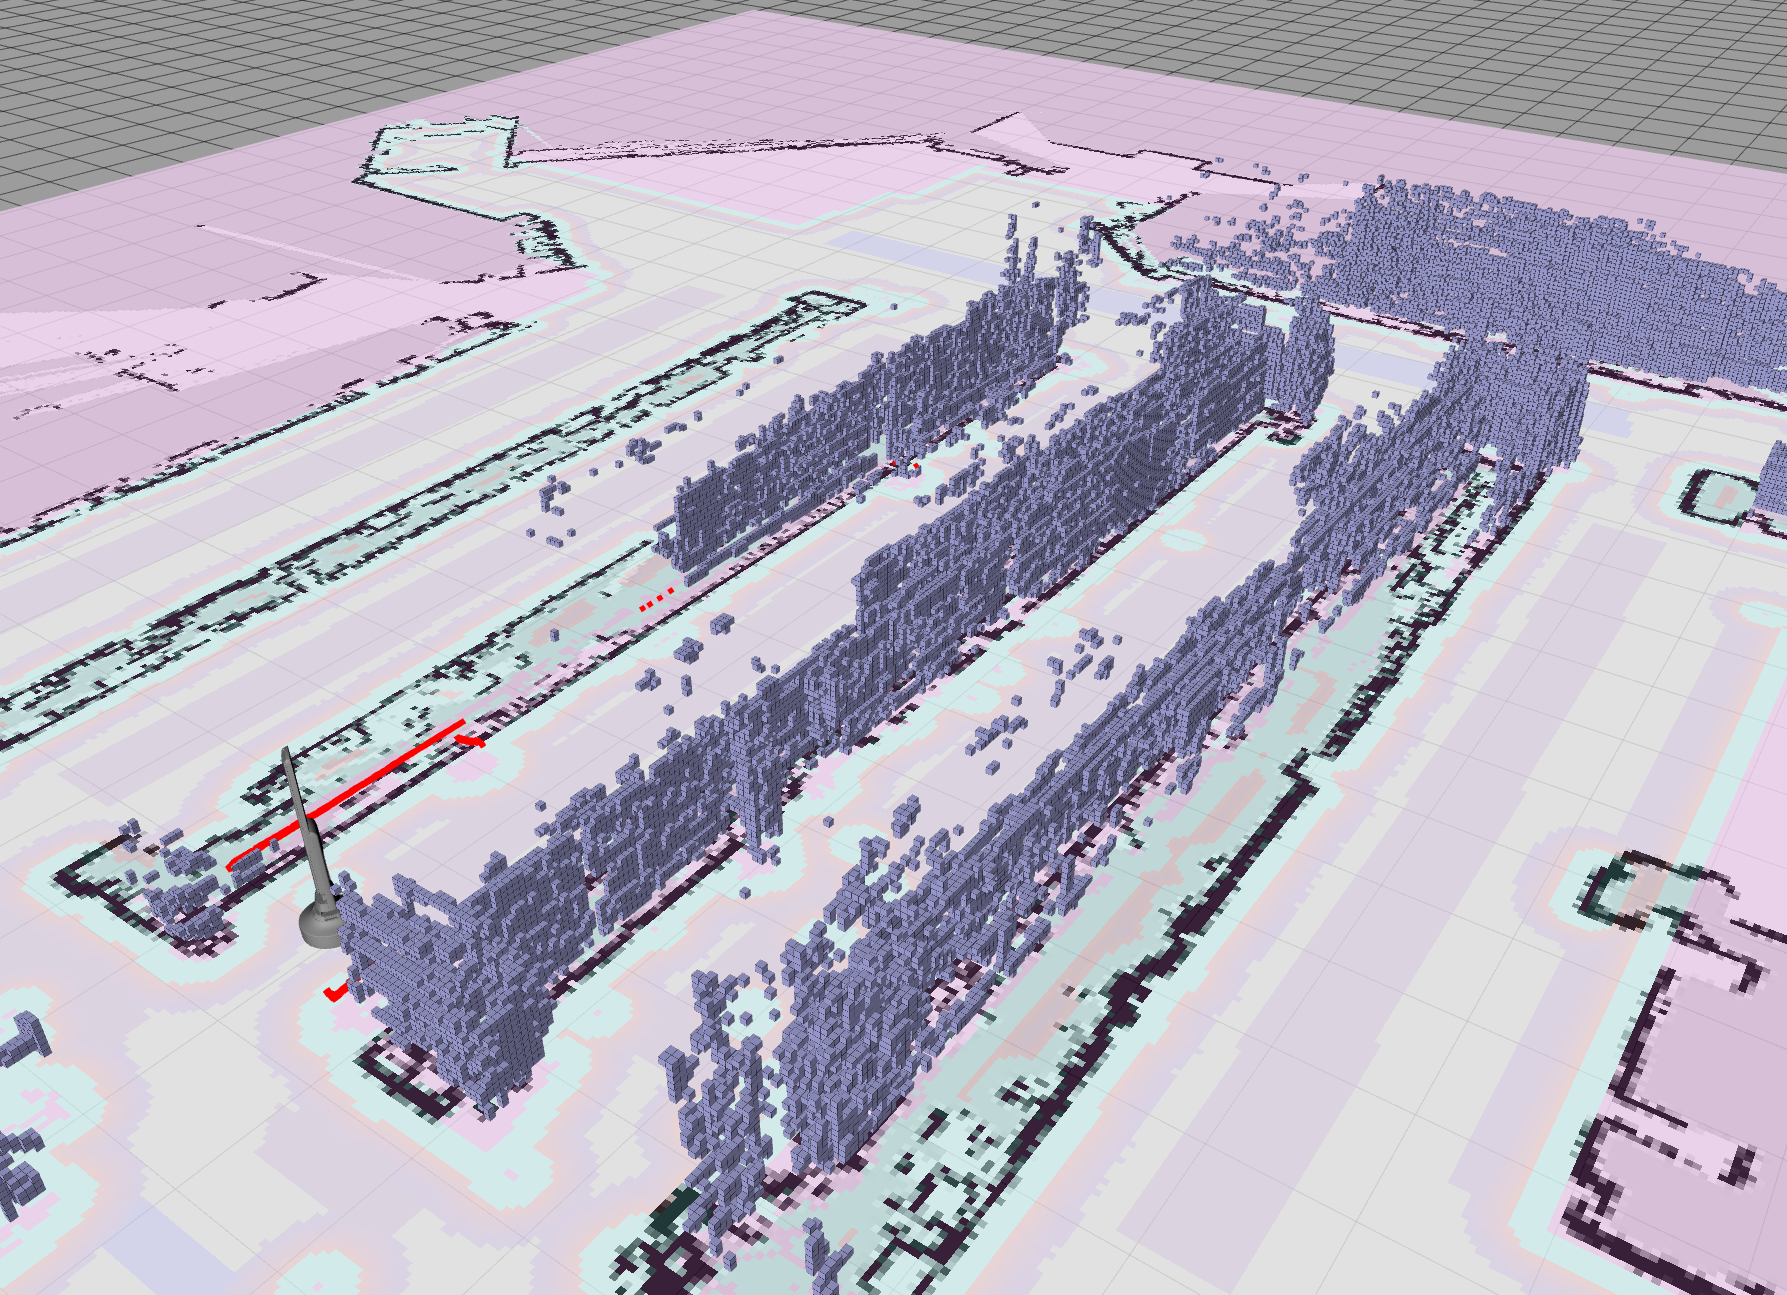
\includegraphics[width=0.8\textwidth]{c4_06.png}
    \caption{STVL in action in a dynamic and cluttered warehouse environment}
    \label{fig:stvl}
\end{figure}


\subsection{Optimal DDS configuration}

In the initial stages of the experimental activities, we encountered various issues related to the LiDAR. 
Such as low message frequency, significant gaps in measurement production, and crashes in the applications.
This would lead the robot not to navigate correctly, and often not perceiving the obstacles in the immediate vicinity.
Overall Nav2 was not reliable and robust, especially in dynamic and cluttered environments.
Figure \ref{fig:3dlidar} shows the pointcloud generated from the 3D LiDAR sensor in a cluttered environment.
When the sensor is working correctly, it can provide a detailed and accurate representation of the environment,
at a constant and stable frequency. However, the LiDAR sensor was not working correctly, so the pointcloud data
was received with gaps and delays.

\begin{figure}[t]
    \centering
    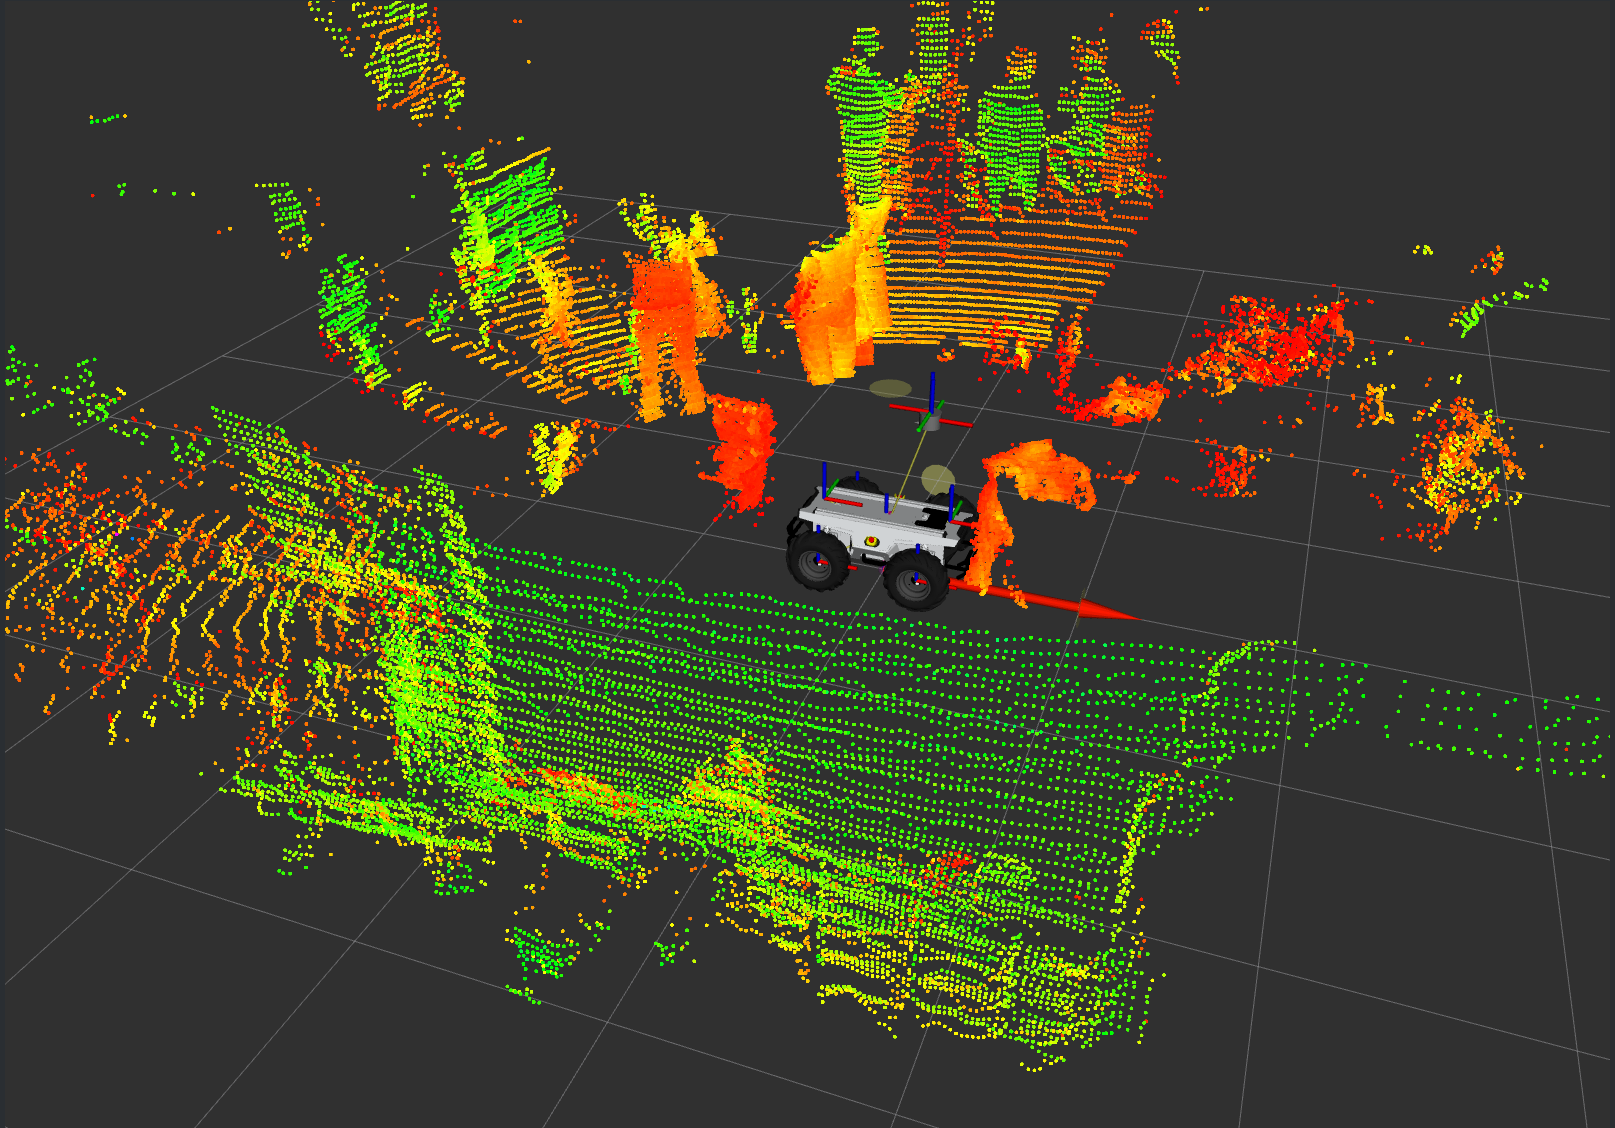
\includegraphics[width=1.0\textwidth]{c4_18.png}
    \caption{3D LiDAR sensor in a cluttered environment}
    \label{fig:3dlidar}
\end{figure}

The LiDAR sensor, integral to localization and obstacle avoidance algorithms, exhibited low and unreliable frequency,
ranging from 3Hz to 8Hz, instead of its nominal 10Hz.  This variability, primarily attributed to the combined 
effects of the router connecting the robot to the network and the default Data Distribution Service (DDS) middleware 
configuration within ROS2, caused significant disruptions to the software's operation.

The DDS middleware, configured to broadcast all ROS2 packets to the laboratory network, introduced delays and packet loss
due to the network's inability to handle the high-frequency, heavy-weight LiDAR data streams.  
This unreliability in data transmission not only affected the LiDAR sensor but also tampered with the proper 
initialization and function of the IMU sensor used in SLAM algorithms.

To resolve these issues, the DDS middleware was meticulously reconfigured to ensure that all ROS-related nodes
and data streams remained local to the robot's computer, preventing them from traversing the router and laboratory network.
This change effectively eliminated the broadcast-induced delays and packet loss.  Additionally, ROS2 was configured
to utilize the Cyclone DDS middleware, a lightweight and fast implementation particularly suited for real-time, 
high-frequency heavy-data transmission. Cyclone DDS proved capable of reliably handling the heavy LiDAR data packets
at high frequencies, ensuring their complete and timely transmission.

Following these configuration changes, the LiDAR sensor consistently delivered a stable scan rate of 10Hz,
resolving the software crashes and malfunctions previously observed. The system was further tested with the
LiDAR operating at a higher frequency of 20Hz with lower resolution, and stability was maintained.

This solution not only fixed the immediate LiDAR frequency issue but also had cascading positive effects on other
system components. The IMU sensor, crucial for the SLAM algorithm, was now able to initialize correctly with a stable
LiDAR data stream, eliminating odometry drift. Numerous other algorithms and software components benefited from the 
improved data reliability, resulting in robust and reliable navigation performance for autonomous tasks.

The Cyclone DDS configuration file, shown in \ref{lst:cyclone}, establishes settings for a domain with ID "any,"
indicating it can participate in any DDS domain. It restricts communication to the local loopback interface ("lo") 
and explicitly disables multicast for both discovery and data transmission. This configuration also allows
Cyclone to automatically assign unique identifiers to participants within the domain. 
For peer discovery, it targets only the local machine ("localhost").
This configuration prioritizes local, unicast communication and controlled participant identification.

\begin{lstlisting}[language=XML, caption=Cyclone DDS configuration file, label=lst:cyclone, float=t]
    <CycloneDDS xmlns="https://cdds.io/config" 
        xmlns:xsi="http://www.w3.org/2001/XMLSchema-instance">
        <Domain id="any">
            <General>
                <Interfaces>
                    <NetworkInterface name="lo"/>
                </Interfaces>
                <AllowMulticast>false</AllowMulticast>
            </General>
            <Discovery>
                <ParticipantIndex>auto</ParticipantIndex>
                <Peers>
                    <Peer Address="localhost"/>
                </Peers>
                <MaxAutoParticipantIndex>120</MaxAutoParticipantIndex>
            </Discovery>
        </Domain>
    </CycloneDDS>
\end{lstlisting}


\section{Parking Algorithm for Mobile Robot}
\label{sec:parking}

A \textbf{parking algorithm} was designed for the mobile robot to autonomously approach the target location
to better perform manipulation activities.
The parking algorithm takes as input the location in the map of the target spot that the robotic arm must reach,
and it outputs the optimal parking pose to give the robotic arm
enough space to reach the target. The algorithm is designed and structured to ensure that the mobile robot
can park in a position where the robotic arm can interact with the target object, without colliding with 
the obstacles in the environment nor with the target object itself. The mobile robot must park so that it 
faces the opposite direction of the target object because the robotic arm is mounted on the back of the robot.

The parking algorithm considers both the robot's footprint and uses a heuristic to approximate the robotic arm's
reachability constraints to ensure that the robot can park in a position where the robotic arm should be able 
to reach the target object. This heuristic does not guarantee that the robotic arm can always reach the target object,
but it works as a good approximation of the robotic arm's workspace.
The algorithm also considers the costmap generated by Nav2 to compute the optimal parking
pose that minimizes the cost of the footprint, meaning that the robot will be the furthest possible from
the obstacles in its vicinity. 

The parking algorithm is then used by the Nav2 commander APIs to send the parking pose as a ROS2 action goal,
which generates a collision-free path for the robot to follow to reach the parking pose. The robot then executes
the planned trajectory and parks near the computed parking pose. While the mobile robot navigates
autonomously to the parking pose, it publishes feedback data containing its current position and its distance 
from the parking pose. 

The parking algorithm is non-deterministic, meaning that it can compute different parking poses for the same target
pose, depending on the obstacles in the environment. The algorithm's pseudocode is displayed in \ref{alg:parking}.

\begin{algorithm}[H]
    \caption{\textbf{Parking Pose Computation Algorithm}}
    \label{alg:parking}
    \begin{algorithmic}[1]
    \Require Target $t = (x_t, y_t, \theta_t)$
    \Require Costmap $C$, Robot's Footprint $F$

    \State $n \gets 50$ \Comment {number $n$ of parking pose candidates $p_c$}
    \State $r \gets 0.4$ \Comment {parking radius in meters from the target position}
    \State $P_{current} \gets$ current robot's position in the map
    \State $V_c \gets \emptyset$  \Comment{list of valid candidate poses}

    \Function{rank}{$p$}
        \State $w_{cost} = 0.5, w_{dist} = 0.2, w_{orientation} = 0.3$ 
        \State $cost = cost(F(p), C)$ \Comment{cost in the costmap for given pose and footprint}
        \State $dist = ||P_{current} - p|| ^2$ \Comment {Euclidean distance between poses}
        \State $orient = | \theta_t - \theta_p |$ \Comment {difference between target and candidate orientation}
        \State \Return $w_{cost} \cdot cost + w_{dist} \cdot dist + w_{orientation} \cdot orient$
    \EndFunction

    \For {$i = 1$ to $n$}
        \State $\phi \sim $\textit{Uniform}$(-\phi_{max}, \phi_{max})$ \Comment {random angle}
        \State $x_c \gets x_t + r \cdot \cos(\theta_t + \phi)$ \Comment {candidate $x$ coordinate}
        \State $y_c \gets y_t + r \cdot \sin(\theta_t + \phi)$ \Comment {candidate $y$ coordinate}
        \State $\psi \sim $\textit{Uniform}$(-\psi_{max}, \psi_{max})$ \Comment {random orientation}
        \State $\theta_c \gets \theta_t + \psi$ \Comment {candidate orientation}
        \State $p_c \gets (x_c, y_c, \theta_c)$ \Comment {candidate parking pose}
        \State \Comment{ discard the poses having their footprint $F$ with lethal cost in costmap $C$}
        \If {\textit{cost}$(C, F(p_c)) \neq $ \textit{LETHAL}}
            \State add $p_c$ to $V_c$
        \EndIf
    \EndFor
    \State $V_{ranked} \gets \left[\textbf{rank}(p_{c,1}), \ldots, \textbf{rank}(p_{c, n_c})\right] 
        \quad \forall p_c \in V_c $
    \State $V_{c} \gets \textit{sorted}(V_{ranked}, V_c) $ \Comment{sort list of candidates by their rank}

    \Repeat 
        \State pick {$P_{candidate} \in V_c$} \Comment{pick parking pose from the highest ranked candidates}
        \If {$\exists$ traversable path from $P_{current}$ to $P_{candidate}$}
            \State save parking pose $P_{parking} \gets P_{candidate}$
        \EndIf
    \Until {a traversable path is found}
    \If {$\exists P_{parking}$}
        \State \textbf{navigate} towards $P_{parking}$ with computed traversable path
    \EndIf
    \end{algorithmic}
\end{algorithm}

The algorithm \ref{alg:parking} prioritizes poses that are closer to the target, have lower costs in the costmap, 
and are aligned with the target orientation. The use of random sampling allows for exploring a variety of potential parking spots.
It also ensures that the chosen parking pose is reachable by checking for a traversable path.
The algorithm uses the following inputs and parameters:
\begin{itemize}
    \item $t$: the target pose (final position and orientation): $(x_t, y_t, \theta_t)$.
    \item $C$: the costmap: grid-based representation of the environment, where each cell has a cost associated with it.
    \item $F$: the robot's footprint: shape and size of the robot, which is used to check for collisions with obstacles.
    \item $n$: the number of parking pose candidates to generate (default: $50$)
    \item $r$: the parking radius around the target position (default: $0.4$ meters)
\end{itemize}

The algorithm \ref{alg:parking} consists of the following steps:

\begin{enumerate}
    \item \textbf{Rank Function} definition: A function that evaluates the quality of a candidate pose 
    based on cost, distance, and orientation. It calculates a weighted sum of these factors: 
    cost (based on the costmap), distance (from the current position), and orientation 
    (difference from the target pose). The weights determine the relative importance of each factor.
    \item \textbf{Candidate Generation and Filtering}: The algorithm iterates $n$ times to generate candidate poses:
        \begin{enumerate}
            \item A random angle ($\phi$) is chosen within specified limits.
            \item The candidate pose's $x$ and $y$ coordinates ($x_c, y_c$) are calculated based on the target position,
            parking radius, and random angle.
            \item A random orientation ($\psi$) is chosen within limits.
            \item The candidate orientation ($\theta_c$) is calculated.
            \item The candidate pose ($p_c$) is formed using ($x_c, y_c, \theta_c$).
            \item The cost of the robot's footprint at $p_c$ is checked. If it's not lethal 
            (i.e., not colliding with an obstacle), $p_c$ is added to the list of valid candidates ($V_c$).
        \end{enumerate}
    \item \textbf{Ranking and Sorting}: The rank function is applied to each valid candidate pose in $V_c$. 
    The list of candidates ($V_c$) is sorted in ascending order based on their ranks (lower rank is better).
    \item  \textbf{Path Planning and Navigation}: The algorithm repeatedly picks the highest-ranked candidate pose from $V_c$.
    It checks if a traversable path exists from the current position ($P_{current}$) to the candidate pose. 
    If a path is found, the candidate pose is saved as the parking pose ($P_{parking}$). 
    This process continues until a traversable path is found or all candidates are exhausted.
    \item \textbf{Navigation (if applicable)}: If a suitable parking pose ($P_{parking}$) is found, 
    the robot navigates towards it using the computed traversable path.
\end{enumerate}

Experimental tests were performed to evaluate the accuracy and reliability of the parking algorithm.
The tests were conducted in both simulated and real environments, with different configurations of obstacles
and target poses. The parking algorithm was able to compute effective parking poses in most cases,
but it struggled with tight spaces and narrow passages, where the robot had limited space to park.
The biggest limitation of this algorithm is that it \textbf{does not consider the exact feasible workspace} of the robotic arm
when computing the parking pose, which can lead to the robot parking in a position where the robotic arm
cannot reach the target object. It instead uses a heuristic to approximate the robotic arm's workspace,
which is not always accurate, leading to suboptimal parking poses in some cases.
This limitation is due to the impossibility of predicting the cartesian
target pose that the cobot will have to reach, as it depends on the object's position and orientation
in the environment. The parking algorithm is a good starting point for further development and improvement
to address these limitations and ensure that the robot can park in a useful position also for the robotic arm.

Despite the parking algorithm being effective in most cases, there were some cases where the robot parked too close
or too far from the object where the robotic arm would interact. This was mainly due to the
\textbf{imprecision of the localization algorithm} and the local planner's inability to reach the exact parking pose,
especially in tight spaces. This problem resulted in a precision error 
in the final position of the robot, in the range of $\pm 15$cm from the desired parking pose. This problem was
critical because an error of just a few centimeters could result in the robot being too close to the object
to find it or interact with it, or too far. Since no ideal solution exists that
can compensate for the localization and navigation errors, a workaround was implemented. When the robot cannot interact 
with the object because of the distance to it, the robot chooses and navigates to a different parking pose,
and tries to interact with the object from the new position. 

\section{ArUco Marker Detection and Pose Estimation}
\label{sec:multiaruco}

ArUco markers are square markers with unique black-and-white patterns that can be easily detected
and identified by computer vision algorithms.
Detecting and estimating the pose of an ArUco marker from an image involves a two-step process.
First, the ArUco marker is detected in the image using the ArUco library available in OpenCV. 
This library provides functions to detect various ArUco dictionaries and families. 
Once detected, the marker's corners are extracted, and its unique ID is identified. 
The second step involves estimating the pose of the ArUco marker, which refers to its position 
(translation vector) and orientation (rotation vector) with respect to the camera. The function for pose estimation 
takes the detected marker corners, the marker size, and the camera's intrinsic parameters (i.e. focal length,
principal point, and distortion coefficients) as input and returns the pose of the marker in the form of a rotation
vector and a translation vector.

The intrinsic parameters of the camera are crucial for accurate pose estimation. These parameters describe the camera's
internal characteristics, such as the focal length, which determines the field of view, and the principal point,
which is the center of the image. The distortion coefficients model the lens distortion, which can cause straight
lines to appear curved in the image. By incorporating these parameters into the pose estimation process,
we can compensate for the camera's inherent distortions and obtain a more accurate estimate of the ArUco marker's pose
in the real world. It was also necessary to calibrate the camera's intrinsic parameters using a checkerboard
calibration pattern and the automatic calibration software tool provided by the RealSense SDK.

The dictionary for the ArUcos used throughout the project is the 4x4. It is useful for locating the marker signaling
the control panel from a distance, instead of the 7x7 dictionary markers initially used.
The 4x4 markers require fewer pixels to be represented, therefore the minimum area of pixels required
for detection is smaller. This implies that the 4x4 markers can be detected from a greater distance than the 7x7 markers.

\subsection{Multi-ArUco Plane Estimation Algorithm}

One of the challenges faced was estimating with precision the orientation of small ArUco markers from the camera feed.
The pose estimation algorithm works well for markers that appear large in the image, but it struggles with
the ones that appear smaller due to the size and distance from the camera. The estimation of the orientation
was the most challenging part, as the pose estimation algorithm often returns orientation values that
oscillate between different values, making it difficult to determine the correct orientation of the marker.
To address this issue, a multi-ArUco plane estimation algorithm was designed for estimating the orientation of a plane over which
multiple ArUco markers are placed. Figure \ref{fig:multi_aruco} shows the algorithm in action.

\begin{figure}[t]
    \centering
    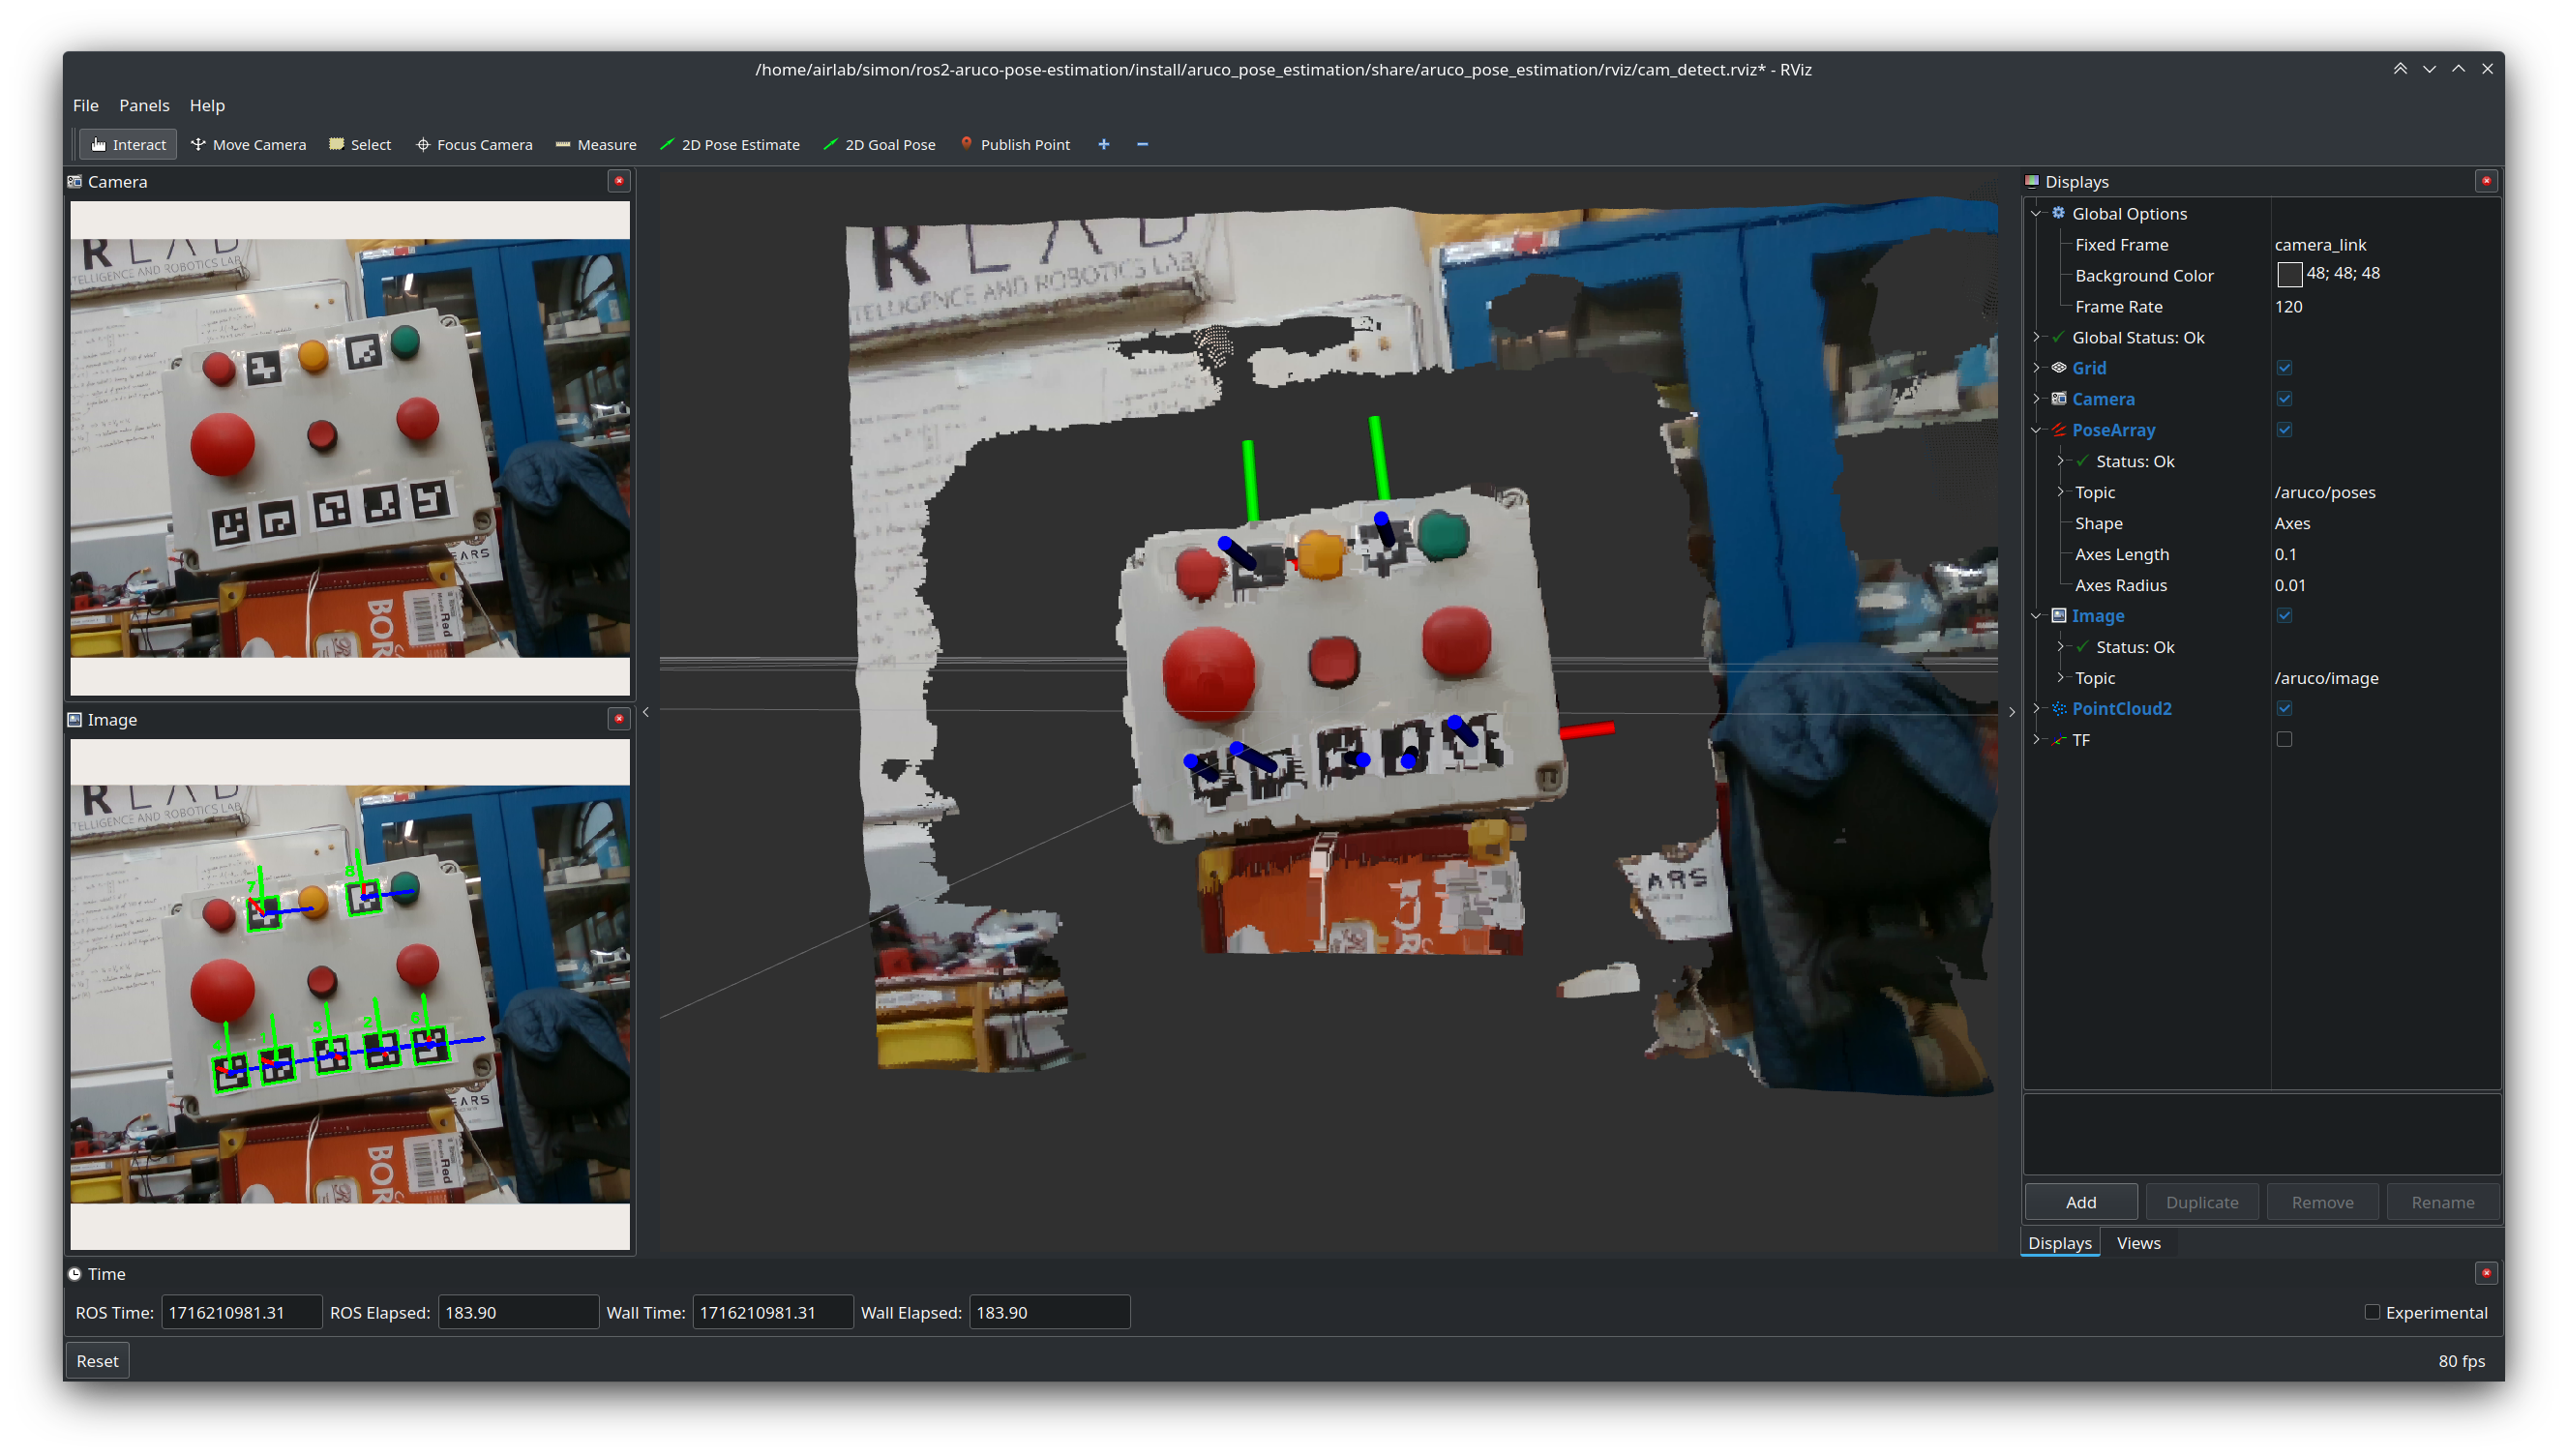
\includegraphics[width=1.0\textwidth]{c4_17.png}
    \caption{Multi-ArUco Plane Estimation algorithm in action. The screenshot shows RViz2 displaying
    on the top left corner the input image, the bottom left the image with the detected markers drawn on top of it,
    and in the center the colored pointcloud captured by the depth sensor.}
    \label{fig:multi_aruco}
\end{figure}

The algorithm works by detecting multiple ArUco markers in the image and estimating their poses using the pose
estimation algorithm. The poses of the ArUco markers are then used to estimate the orientation of the plane
on which the markers are placed. The algorithm assumes that the ArUco markers are \textbf{coplanar}, meaning that 
they have different positions but the same orientation. By estimating the orientation of the plane that passes
through the markers, we can determine the correct orientation of the markers from the vector normal
to the plane. The algorithm processes a list of ArUco markers poses and returns the poses with their
estimated orientation, meaning that all processed poses share the same orientation value.

The algorithm makes use of the following statistical data analysis techniques:

\begin{itemize}
    \item \textbf{RANSAC (Random Sample Consensus)}: RANSAC is an iterative algorithm used to estimate
    the parameters of a mathematical model from a set of observed data points that contain outliers.
    RANSAC works by randomly selecting a subset of data points and fitting a model to them. The model is then
    evaluated against the remaining data points, and the points that are consistent with the model are considered
    inliers. The process is repeated multiple times to find the best-fitting model with the maximum number of inliers.
    RANSAC is used to discard the outlier data points observed in the ArUco markers' poses.
    \item \textbf{Least Squares Estimation (LSE)}: LSE is a mathematical method used to find the best-fitting curve
    that minimizes the sum of the squared differences between the observed data points and the model's predictions.
    LSE is used by the RANSAC model to fit the plane that passes through the ArUco markers' poses.
    \item \textbf{Principal Component Analysis (PCA)}: PCA is a statistical method that identifies patterns
    in data by transforming it into a new coordinate system, where the data points are uncorrelated.
    PCA is used to find the principal components of the data, which are the directions of maximum variance.
    In the context of this algorithm, PCA is used to find the vector passing through points lying on a line.
    It is used as a technique for outlier removal and noise reduction in the data.
    \item \textbf{Singular Value Decomposition (SVD)}: SVD is a matrix factorization technique that decomposes
    a matrix into three matrices, which represent the singular vectors and singular values of the original matrix.
    SVD is used as an optimization technique to find the best-fitting plane that passes through the given points.
    It works as a technique for reducing the dimensionality of the data, by reducing the impact of noisy
    and irrelevant data points.
\end{itemize}

The perception algorithm works as illustrated in \ref{alg:multi_aruco}. The points used as input for the algorithm
are the 3D coordinates of the ArUco markers detected in the image. 

\begin{algorithm}[H]
    \caption{\textbf{Multi-ArUco Plane Estimation Algorithm}}
    \label{alg:multi_aruco}
    \begin{algorithmic}[1]
    
    \Require points $P = \left[ p_1, \ldots, p_n \right]$ with $p_i = (x_i, y_i, z_i)$ coordinates of all points
    \Require collinear points $T = \left[t_1, \ldots, t_n \right]$ with $t_i = (x_i, y_i, z_i)$ assumed to be collinear
    
    \Function{RANSAC}{P}
        \State $\tau \gets 0.01$ \Comment {distance threshold in meters}
        \Repeat
            \State $S =$ random subset of points from $P$
            \State $c =$ centroid($S$) 
            \State $n = SVD(S - c)$  \Comment{Compute SVD from subset of points centered in $0$}
            \State inliers $ = 0$ \Comment{number of inliers for S}
            \ForAll { $s_i$ in $S$}
            \State $d = n \cdot s_i$ \Comment{distance between normal $n$ and point $s_i$}
                \If { $||d|| ^2 < \tau$} \Comment{if point $s_i$ is close enough to the plane defined by $n$}
                    \State inliers $++$
                \EndIf
            \EndFor
        \Until {inliers number is maximized}
        \State \Return $n$ \Comment{Returns normal vector $n$ to the best fitting plane to $S$}
    \EndFunction
    \State
    \State $n$ = \textbf{RANSAC}$(P)$
    \State $c =$ \textit{centroid}($T$) 
    \State $B = $ \textbf{PCA}$(T)$ \Comment{compute \textbf{PCA} of collinear points without centroid}
    \State $d = B[2]$ \Comment{direction of highest variance is the last eigenvector in $B$}
    \State $V_x \gets d, \quad V_z \gets n$
    \State $V_y \gets V_z \times V_x$ 
    \State $Rot = \left[V_x, V_y, V_z \right]$ \Comment{compose 3d rotation matrix from vectors}
    \State $q = $ \textit{rot2quat}$(Rot)$ \Comment{convert rotation matrix to quaternion $q$}
    \State update points in $P$ with the orientation quaternion $q$
    \end{algorithmic}
\end{algorithm}

The algorithm \ref{alg:multi_aruco} requires the following inputs:
\begin{itemize}
    \item $P$: A set of 3D points ($x, y, z$ coordinates) from the list of detected ArUco markers estimated poses,
    assumed to be all on the same plane (coplanar).
    \item $T$: A subset of points from $P$ that are known to be collinear.
\end{itemize}

The algorithm consists of the following steps:

\begin{enumerate}
    \item \textbf{RANSAC Plane Fitting}: The RANSAC function is applied to the full set of points ($P$) 
    to obtain the normal vector ($n$) of the plane.
        \begin{enumerate}
            \item Initialization: A distance threshold ($\tau$) is set to determine how close points need to be to a plane
            to be considered inliers.
            \item Iteration: The algorithm iteratively performs the following:
                \begin{enumerate}
                    \item A random subset of points ($S$) is selected from $P$.
                    \item The centroid ($c$) of $S$ is calculated.
                    \item Singular Value Decomposition (\textbf{SVD}) is applied to $S$ after centering it around the origin. 
                    This yields a normal vector ($n$) representing the best-fitting plane to $S$.
                    \item The number of inliers is counted. Inliers are points from $S$ whose distance to the plane 
                    defined by $n$ is less than $\tau$.
                \end{enumerate}
            \item Termination: The loop continues until the maximum number of inliers is found.
            \item Output: The normal vector ($n$) of the best-fitting plane is returned.
        \end{enumerate}

    \item \textbf{Plane Orientation Refinement}:
        \begin{enumerate}
            \item Normal Calculation: The RANSAC function is applied to the full set of points ($P$) to obtain
            the normal vector ($n$) of the plane.
            \item Centroid Calculation: The centroid ($c$) of the collinear points ($T$) is calculated. 
            The centroid is removed from the points to ensure that the plane passes through the origin.
            \item Direction Vector: Principal Component Analysis (PCA) is performed on $T$, and the eigenvector corresponding
            to the highest eigenvalue is selected as the direction vector ($d$). This vector lies within the plane
            and represents the direction of greatest variance among the collinear points.
            \item Coordinate Frame Construction: An orthonormal basis is constructed:
                \begin{itemize}
                    \item $V_x$: The direction vector ($d$).
                    \item $V_z$: The plane's normal vector ($n$).
                    \item $V_y$: The cross product of $V_z$ and $V_x$.
                \end{itemize}
            \item Rotation Matrix and Quaternion: The basis vectors are used to create a rotation matrix 
            ($Rot$), which is then converted to a quaternion ($q$). This quaternion represents the orientation of the plane.
        \end{enumerate}

    \item \textbf{ArUco Markers Poses Update}: The points in $P$ are updated by applying the rotation quaternion ($q$) 
    to align them with the estimated plane orientation.
    \item \textbf{Output}: The algorithm produces a quaternion ($q$) that describes the orientation of the plane in 3D space.
    All ArUco markers' poses are updated with this orientation, ensuring that they share the same orientation.
\end{enumerate}


\section{Object Detection with YOLOv8}
\label{sec:yolov8}

% Add the architecture diagram
\begin{figure}[H]
    \centering
    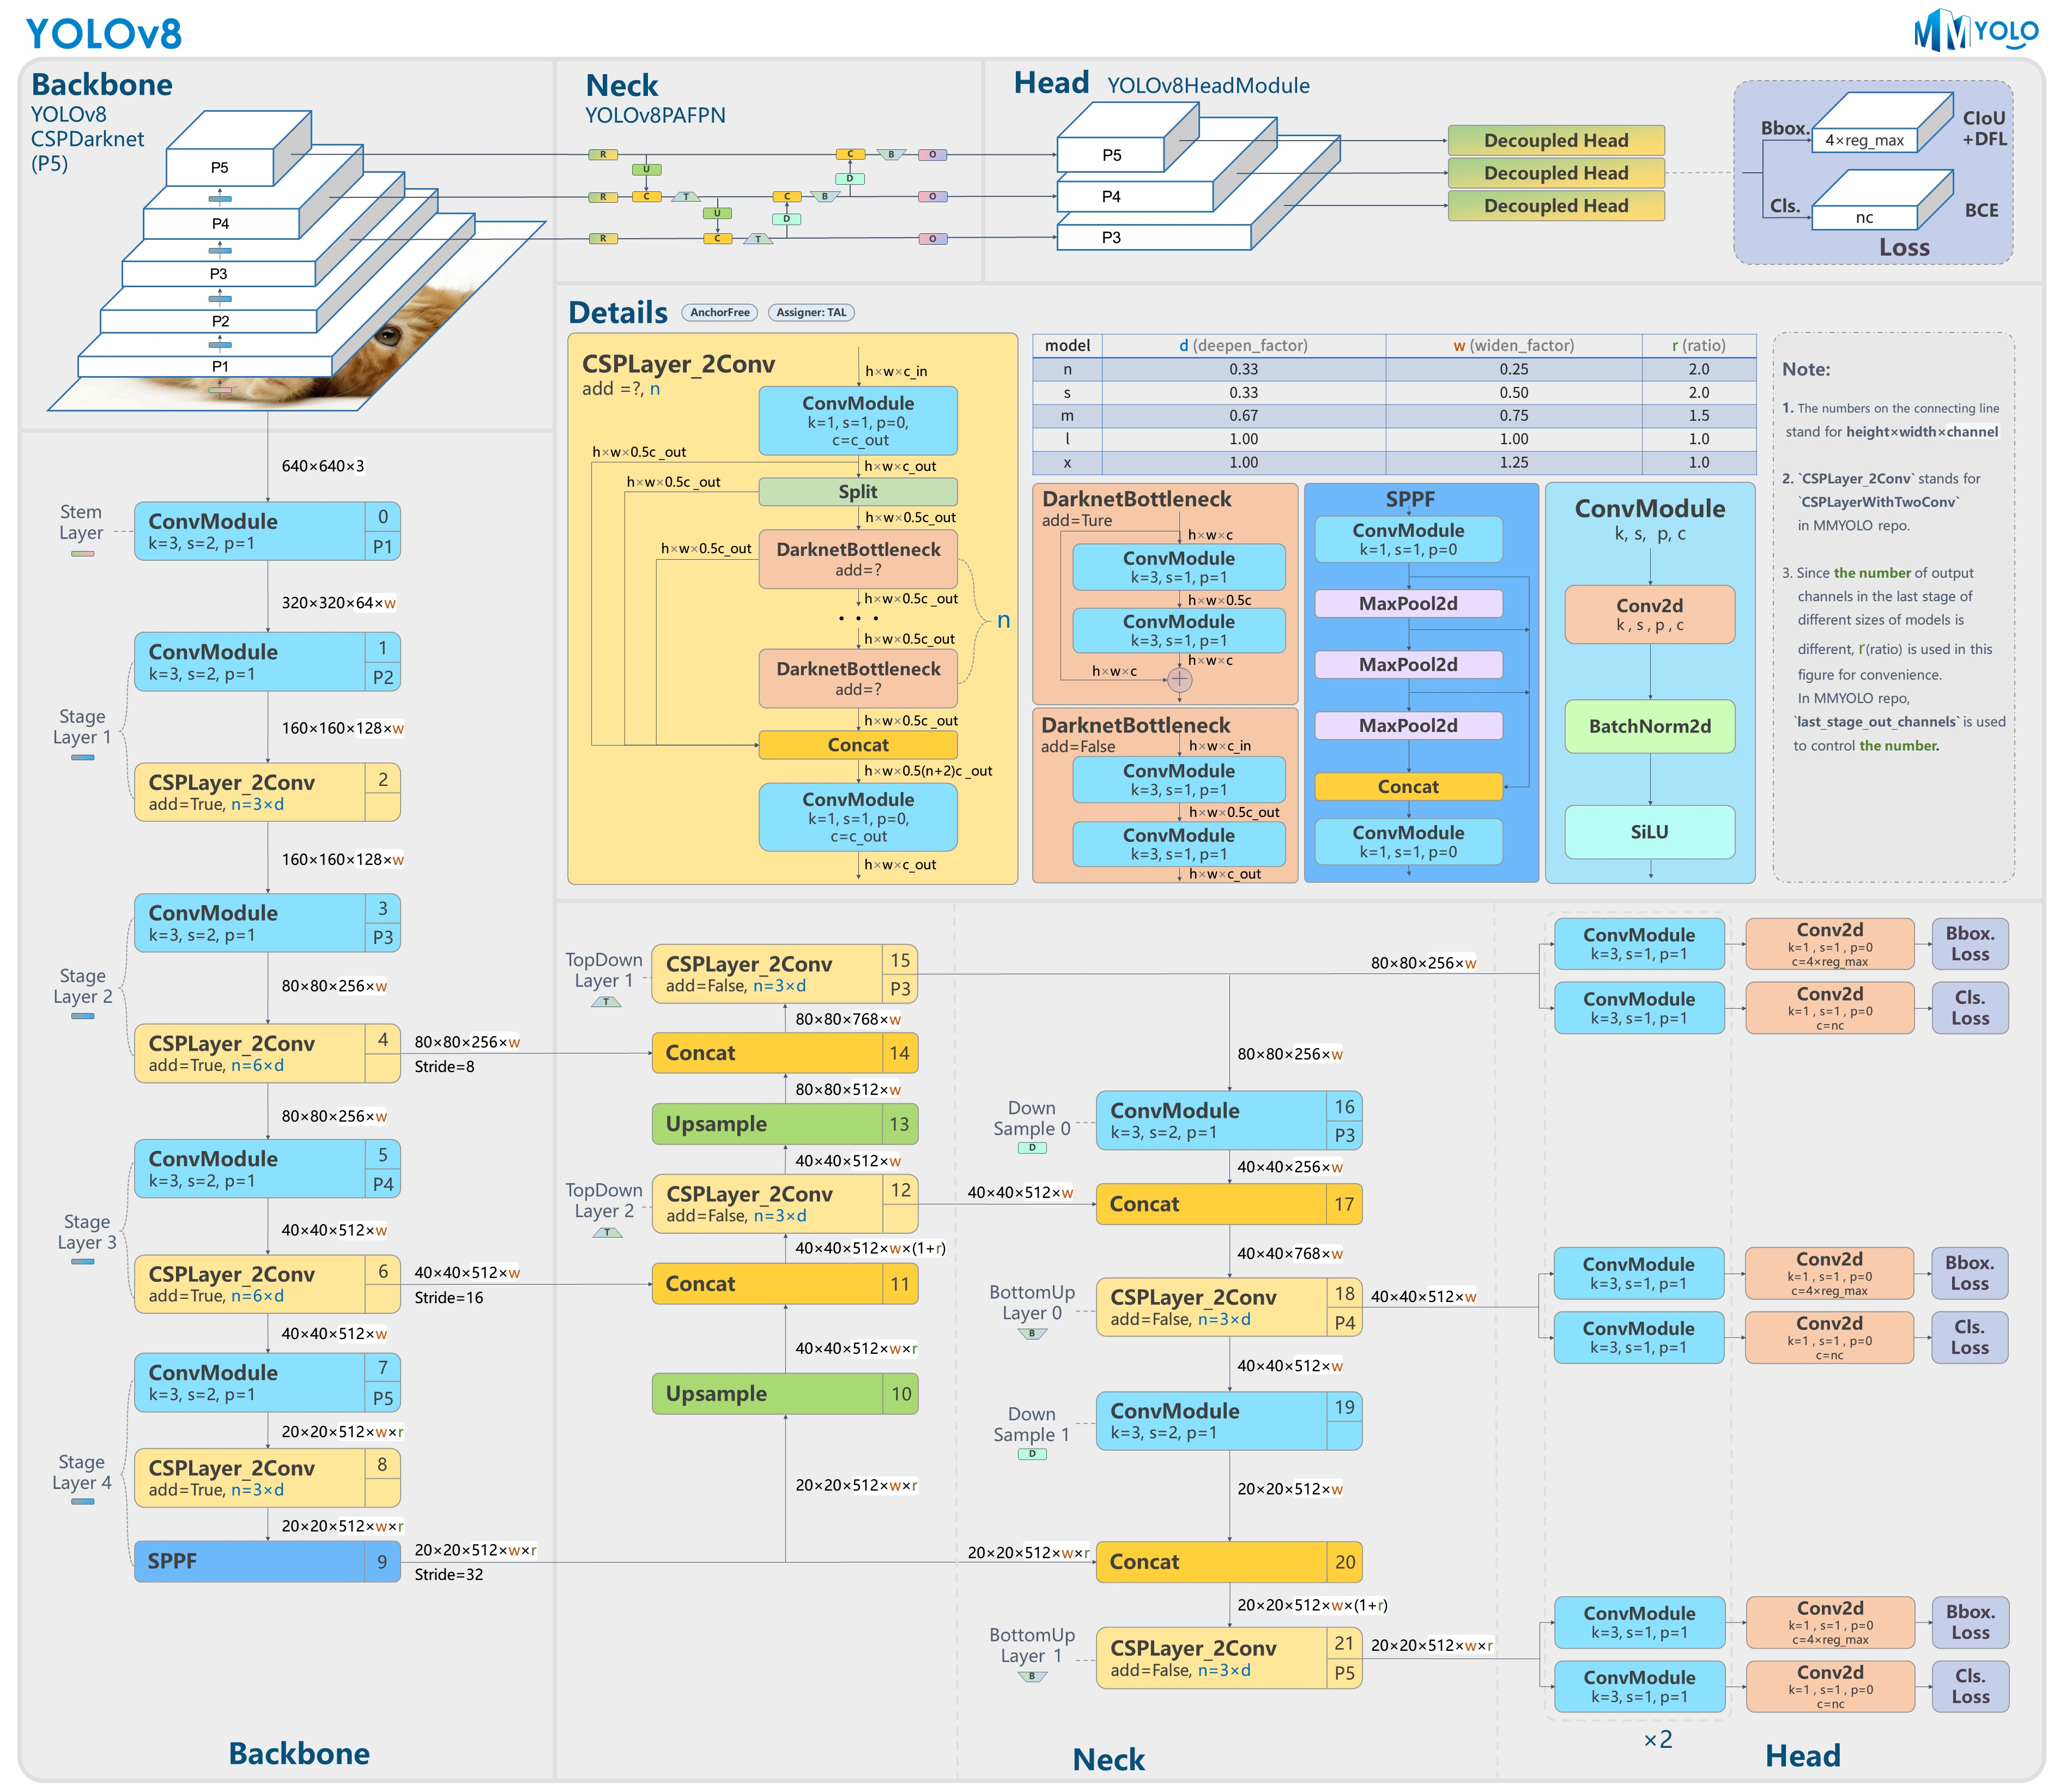
\includegraphics[width=1.0\textwidth]{c4_10.jpg}
    \caption{Architecture overview in detail of the YOLOv8 architecture}
    \label{fig:yolov8}
\end{figure}

For the project, it was also necessary to detect objects in the environment, such as colored balls and apples, which the robot
had to grasp and move to a different location. For this task, YOLOv8 object detection is employed, trained
on a custom dataset. Figure \ref{fig:balls} shows the YOLOv8 model in inference
in realtime, predicting the colors of the balls in the field of view of the camera.

\textbf{YOLO (You Only Look Once)} is a cutting-edge, real-time object detection algorithm 
that has revolutionized computer vision \cite{redmon2015yolo}.
Unlike traditional methods that require multiple passes over an image, YOLO analyzes the entire image in a single pass,
making it fast and efficient. It divides the image into a grid and predicts bounding boxes and class probabilities
for each grid cell simultaneously, achieving high accuracy while maintaining speed. 
YOLO has evolved through several versions (YOLOv2, YOLOv3, etc.), each improving upon the previous iteration in terms of speed, 
accuracy, and ability to detect small objects. Its versatility and effectiveness have led to widespread adoption in various
applications, including autonomous driving, robotics, and image analysis tools. This was the object detection neural
network of choice for the project, as it provided the speed and accuracy needed for detecting objects in real-time
from the camera feed. It is also lightweight, making it ideal to run on CPUs without the need for a GPU.
The inference time for a single image on an Intel i7 12th gen CPU was around $0.15$ seconds, which is fast enough
for the time requirements of the application. However, when running along other ROS2 nodes using other CPU-intensive
algorithms, the inference time increased to $0.4$ seconds, which was still acceptable for the demos and tests.

%Add a picture of the detected balls
\begin{figure}[H]
    \centering
    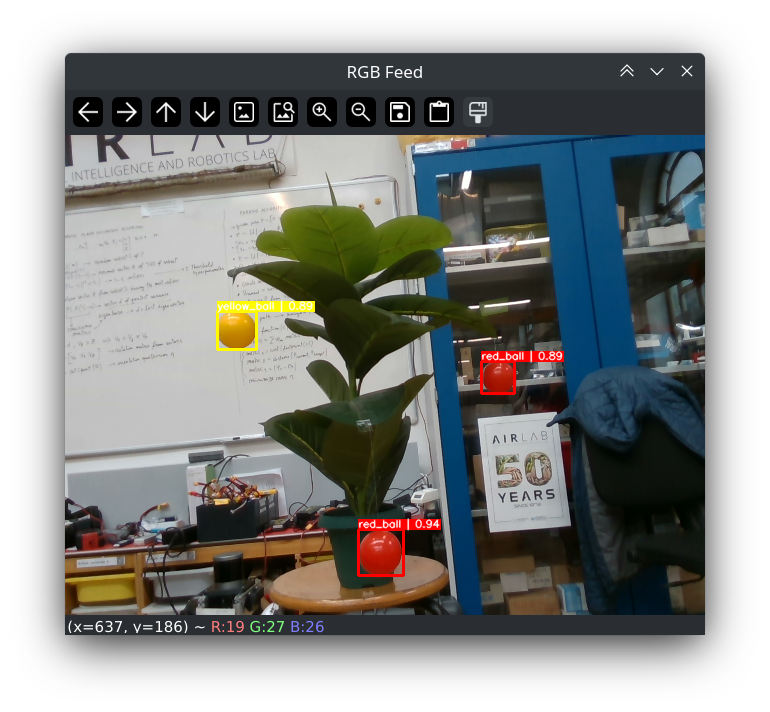
\includegraphics[width=1.0\textwidth]{c4_16.png}
    \caption{YOLOv8 detecting colored balls in realtime from the RGB camera feed. The screenshot displays the image
    with the bounding boxes colored with the same color as the predicted class. For each prediction, the 
    class probability is associated.}
    \label{fig:balls}
\end{figure}

The \textbf{YOLOv8} neural network model is a state-of-the-art object detection model \cite{reis2023realtimeyolov8}
that combines the best features of previous YOLO versions to achieve superior performance. 
This model is used for the object detection task, such as detecting colored balls or apples
from the camera feed. The YOLOV8 architecture is shown in Figure \ref{fig:yolov8}. It shows the backbone architecture
of the YOLOv8 model, which consists of a series of convolutional layers that extract features from the input image
and pass them to the detection head, which predicts the bounding boxes and class probabilities for the objects in the image.
The backbone architecture used in the training is CSPDarknet, which is a state-of-the-art backbone.
The neck is a feature pyramid network (FPN) that combines features from different scales to improve the model's
performance in detecting objects of different sizes.

The YOLOv8 model is trained on a \textbf{custom dataset of colored balls and apples}, which includes images of balls and apples
from different angles, distances, and lighting conditions. The dataset was collected using the RealSense camera mounted
on a tripod, which allowed me to capture images of the objects from different perspectives and distances. The dataset
was annotated manually with the bounding boxes and class labels, which were used to train the YOLOv8 model.
The YOLOv8 model is provided by \textbf{Keras}, a high-level deep-learning library that provides user-friendly
APIs for building and training neural networks. Since the custom training dataset collected is of small size,
data augmentation techniques were employed to increase the dataset's size and diversity, which helped improve the model's
generalization and robustness. The \textbf{data augmentation techniques} included random rotations, translations, and flips
of the images, which created variations of the original images and helped the model learn to detect the balls
from different perspectives and orientations. Many types of image augmentation techniques were included, such as
brightness and contrast adjustments, and Gaussian noise addition, which further increased the dataset's
size and variability. The image augmentation algorithms were implemented using the \textit{Albumentations} library,
a powerful image augmentation library for computer vision tasks, designed for 
object detection tasks. It is essential to properly adjust the bounding boxes after each image
is augmented, to ensure that the bounding boxes are still correctly positioned around the objects of interest.

As training hyperparameters, the batch size is $32$, which is enough for a small dataset,
a learning rate scheduler with exponential decay, and the early stopping callback to stop the training
when the validation loss stops decreasing. The model is compiled with the \textit{Adam} optimizer, which is a popular optimizer
for training deep neural networks, and with the YOLOv8 Backbone, which is a state-of-the-art backbone architecture
that provides the best candidate features for object detection tasks. The metrics used to evaluate the model's performance
are the \textbf{mean Average Precision (mAP)} and the \textbf{Intersection over Union (IoU)},
which are standard metrics for object detection tasks. These metrics are incorporated within the \textit{COCO} evaluation metrics,
which are the standard evaluation metrics provided by the \textbf{KerasCV} library \cite{wood2022kerascv}.

The model is trained with the combination of two loss functions:

\begin{itemize}
    \item \textbf{Box Loss}: The box loss function is used to penalize the model for incorrect predictions of the bounding
    boxes of the objects. The box loss function computes the difference between the predicted bounding boxes and the
    ground-truth bounding boxes, using the \textit{CIoU} (Complete Intersection over Union) loss function, which is a
    state-of-the-art loss function that accounts for the object's aspect ratio and orientation \cite{zheng2021ciou}.
    \item \textbf{Class Loss}: The class loss function is used to penalize the model for incorrect predictions of the
    object classes. The class loss function computes the difference between the predicted class probabilities and the
    ground-truth class labels, using the \textit{Binary Cross-Entropy} loss function, which is the loss function of
    choice for multi-class classification tasks that use multi-hot encoded labels instead of one-hot encoded labels.
    After some tests, the class loss was switched to the \textit{Binary Penalty Reduced Focal CrossEntropy} 
    loss function, a variant of the focal loss function that reduces the penalty for misclassifications, 
    and focuses more on the correct classification of the objects \cite{law2019cornernet}. 
    This loss function helped improve the model's accuracy.
\end{itemize}

The table below \ref{table:metrics} shows the \textbf{evaluation metrics} for the object detection model, which includes
the Average Precision (AP) at different Intersection over Union (IoU) thresholds, the Average Recall (AR),
and the AP for different object sizes (small, medium, large). The Intersection over Union thresholds define
the level of overlap required between the predicted bounding box and the ground-truth bounding box for the prediction
to be considered correct. The AP is a measure of how well the model detects objects across different levels of overlap,
while the AR is a measure of how well the model finds all ground truth objects. The AP and AR are computed for different
object sizes to evaluate the model's performance on objects of different scales. The evaluation metrics provide
insight into the model's accuracy, recall, and generalization capabilities, which are essential for assessing
the model's performance on unseen data.

\begin{table}[t]
    \centering
    \begin{tabular}{|r|c|c|c|}
    \hline
    \textbf{Metric} & \textbf{IoU} & \textbf{Area} & \textbf{Value} \\
    \hline
    AP & 0.50:0.95 & all & 0.452 \\
    AP & 0.50 & all & 0.616 \\
    AP & 0.75 & all & 0.552 \\
    AP & 0.50:0.95 & small & 0.232 \\
    AP & 0.50:0.95 & medium & 0.512 \\
    AP & 0.50:0.95 & large & 0.673 \\
    AR & 0.50:0.95 & all & 0.590 \\
    AR & 0.50:0.95 & small & 0.284 \\
    AR & 0.50:0.95 & medium & 0.659 \\
    AR & 0.50:0.95 & large & 0.780 \\
    \hline
    \end{tabular}
    \caption{Evaluation metrics for the trained YOLOv8 model}
    \label{table:metrics}
\end{table}
    
The table below \ref{table:hyperparameters} shows the hyperparameters and model parameters used in the training
and compiling of the YOLOv8 model. The hyperparameters include the number of epochs, batch size, learning rate,
optimizer, and loss functions used in the training process. The model parameters include the classification loss,
box loss, model size, number of trainable parameters, and the number of classes detected by the model.

\begin{table}[t]
    \centering
    \begin{tabular}{|l|l|}
    \hline
    \textbf{Hyperparameters} & \textbf{Value} \\
    \hline
    Epochs & 42 (Early Stopping) \\
    Batch Size & 32 \\
    Image Size & $640 \times 480$ \\
    Initial Learning Rate & 0.001 \\
    Learning Rate Scheduler & Staircase Exponential Decay \\
    Optimizer & Adam \\
    Momentum & 0.9 \\
    Weight Decay & 0.0005 \\
    Global Clip Norm & 10.0 \\
    Classification Loss & Binary Penalty Reduced Focal CrossEntropy \\
    Box Loss & Complete Intersection over Union \\
    \hline
    \textbf{Model Parameters} & \textbf{Value} \\
    \hline
    Model Size & Small \\
    Trainable Parameters & 14M \\
    Trainable Layers & 4 \\
    Number of Classes & 5 (4 balls, 1 apples) \\
    Prediction Decoder & Multi-Class Non-Maximum Suppression \\
    Confidence Threshold & 0.7 \\
    IoU Threshold & 0.4 \\
    \hline
    \end{tabular}
    \caption{Hyperparameters and model parameters used in YOLOv8 training}
    \label{table:hyperparameters}
\end{table}

One problem faced with this network was the \textbf{high false positive rate} of the trained YOLOv8.
The neural network was trained on a relatively small dataset of images, and it was not able
to generalize well enough to new images. The neural network was detecting objects that were not present in the image,
and this resulted in the algorithm computing grasping poses for objects that were not balls or apples.
This problem was addressed by increasing the threshold for the class confidence score, which is the minimum
confidence score required for the object to be considered a valid detection. By increasing the threshold,
the number of false positives was reduced, and the algorithm became more accurate in detecting the objects
of interest. The threshold is set to $0.7$, which is a good trade-off between accuracy and false positives.

\section{Pose Estimation with Object Detection and Depth Perception}
\label{sec:perception}

The object's pose estimation task involves estimating the position of an object in 3D space using the depth-sensing
camera and the object detection neural network. The object detection algorithm detects the object 
in the RGB image and provides the bounding box coordinates, class label, and confidence score. 
The depth-sensing camera provides the depth map of the scene, which contains the distance of each pixel from the camera.
By combining the object detection results with the depth map, we can estimate the object's position in 3D space
relative to the camera, which is essential for the robot to interact with the object effectively.
The perception algorithm is described in detail in the following section.

This perception algorithm works by creating a \textbf{segmented pointcloud} of the object from the depth map,
using the bounding box coordinates provided by the object detection algorithm, and the projected depth values
from the depth image. This perception algorithm is implemented to estimate the center position
of detected colored balls or apples.
The segmented pointcloud contains only the points that belong to the object, which are used
to estimate the object's position in 3D space. The segmentation process involves extracting the points within
the bounding box and filtering out the points that are not part of the object using a color mask corresponding
to the predicted class label. The segmented pointcloud is then used to estimate the object's center position
by fitting an ideal sphere of known radius to the segmented points, as described in algorithm \ref{alg:sphere}.
This center position is then used to compute the optimal grasping pose for the robot to interact with the object,
as described in algorithm \ref{alg:grasping}.

This perception algorithm is used to estimate the optimal grasping pose for the robot's end-effector to grasp
the object. The algorithm \ref{alg:grasping} works with both colored apples, that have a spherical shape 
with measurable radius, and with apples, that have a more irregular shape. The apples are approximated as spheres
for the grasping pose estimation, and their radius is approximately 5 cm. This value corresponds to half of the
width of the upper part of the apple, which is the part that the robot's end-effector will grasp.

\subsection{Algorithm for Object's Center Estimation}

The algorithm for the object's center estimation from the surface pointcloud is the one described
in \ref{alg:sphere}. This algorithm uses a random sample consensus (\textit{RANSAC}) algorithm to estimate 
the object's center, assuming that the object can be approximated as a sphere of known radius.
The algorithm uses \textit{MLESAC} (Maximum Likelihood Estimation Sample Consensus) to estimate the sphere's center
from the segmented pointcloud. The function used for sphere fitting to a pointcloud is provided by
\textit{SACSegmentation} package from \textit{Pointcloud Library}. This package provides a robust and fast
implementation of the RANSAC algorithm for fitting geometric shapes to pointcloud data. 

\begin{algorithm}[t]
    \caption{\textbf{Sphere Barycenter Estimation from Object Detection}}
    \label{alg:sphere}
    \begin{algorithmic}[1]
    \Require RGB image $I$, Depth image $D$
    \Require predicted bounding box $B = (x, y, w, h)$, predicted class label $\hat{y}$
    \State sphere radius range $r_{min}, r_{max}$, tolerance $\epsilon$
    \State $d_{max} \gets 1.5$ \Comment maximum depth of useful points in meters

    \State $I_{crop} \gets I[y:y+h, x:x+w]$ \Comment Crop the image to the bounding box
    \State $D_{crop} \gets D[y:y+h, x:x+w]$ \Comment Crop the depth image to the bounding box

    \State $P \gets \textit{get\_pointcloud}(D_{crop})$ \Comment Get the pointcloud from the depth image
    \State filter pointcloud $P$ by removing points with $z \geq d_{max}$
    \State $colormask \gets \textit{get\_colormask}(\hat{y})$ \Comment Get the color mask based on predicted class label
    \State $P_{s} \gets \emptyset$ \Comment Object's surface segmented pointcloud
    \For {each pixel $p \in I$}
        \If {color of $p$ is within $colormask$}
            \State $P_{s} \gets P_{s} \cup P(p)$ \Comment Apply color mask filter and add point to surface pointcloud
        \EndIf
    \EndFor

    \State $n_{min} \gets 4$ \Comment minimum number of points passing through a unique sphere
    \For{a fixed number of iterations} \Comment Random sample consensus algorithm
        \State $S \gets$ random subset of $n_{min}$ points from $P_s$  
        \State $c, r \gets$ center and radius of sphere fit to subset $S$
        \If{$r_{min} \leq r \leq r_{max}$}  
            \State Calculate $inliers$: points within a distance threshold $\epsilon$ of the sphere's surface
            \State Calculate \textit{MLESAC} score based on the number of inliers and the residual error
            \If{$score >$ \textit{best\_score}}
                \State Update \textit{best\_model} $\gets (c, r)$, \textit{best\_score} $\gets$ $score$
            \EndIf
        \EndIf
    \EndFor

    \State Refine \textit{best\_model} by fitting the $inliers$ using least squares method

    \State \textbf{return} \textit{best\_model}

    \end{algorithmic}
\end{algorithm}

The algorithm \ref{alg:sphere} works as follows:

\begin{enumerate}
    \item \textbf{Input}: RGB image $I$, Depth image $D$, 
    predicted bounding box $B = (x, y, w, h)$, predicted class label $\hat{y}$
    \item \textbf{Parameters}: Sphere radius range $(r_{min}, r_{max})$, tolerance threshold $\epsilon$,
    maximum depth threshold $d_{max}$.
    \item \textbf{Preprocessing}: Crop RGB and depth images based on object detection bounding box.
    \item \textbf{Pointcloud Generation}: Create a 3D point cloud from the cropped depth image,
    filtering out points beyond a maximum depth threshold.
    \item \textbf{Pointcloud Object Segmentation}: Apply a color mask based on the predicted class label to isolate points
    belonging to the object's surface. The color mask is expressed as a range of HSV values (hue, saturation, value).
    The color used in the mask is equal to the color of the colored ball, or a mix of red and yellow for the apples.
    \item \textbf{RANSAC Sphere Fitting}: Iteratively fit spheres to random subsets of points, evaluating their fit
    based on inlier count and residual error using an \textit{MLESAC} scoring metric. The best-fitting sphere model
    is updated based on the highest score.
    \item \textbf{Model Refinement}: Refine the best-fitting sphere model using least squares optimization on the inliers.
    It will provide a more accurate estimate of the sphere's center and radius.
    \item \textbf{Output}: Return the refined sphere model, representing the estimated center coordinates 
    and estimated radius of the object, within the specified range.
\end{enumerate}


\subsection{Algorithm for Grasp Pose Estimation}

Picking objects requires the software to know where the object is located in the environment and how to grasp it.
Since explicit programming of how to grasp objects is quite difficult and not extensible to different objects,
the algorithm neglects the grasping strategy (meaning the positioning of the fingers on the object)
and focuses on the object's position estimation. The algorithm for
computing the optimal grasping pose focuses solely on the object's center, which is computed from the object's
perceived pointcloud data. This simplification allows the software to be fast in computing the grasping pose,
even though the generated grasping poses are not optimal for all objects. The algorithm is based on the assumption
that the object can be approximated as a sphere and that getting the end effector sufficiently close to the
object's surface is good enough to grasp it.
This simplified approach is acceptable because of the mechanical characteristics of the gripper. 
The silicone fingers are compliant with the shape of the object and account for small variations in shape.

The algorithm used for computing the grasping pose from the object's center is described
in algorithm \ref{alg:grasping}. The object's center is estimated using algorithm \ref{alg:sphere},
using the depth and RGB images. The algorithm generates a list of possible candidate grasping poses
based on the object's center and the object's known radius. For each candidate, it checks whether 
an inverse kinematic solution exists for the end effector at the candidate grasping pose. 
If a solution exists, the candidate grasping pose is added to the list of feasible grasping poses.
The algorithm then uses a heuristic to choose which candidate grasping pose to use, based on the list
of feasible grasping poses. It selects the candidate at one fourth of the list's size. The first candidate in the 
list will correspond to grasping poses of the object from the top, while the last candidate will correspond
to grasping poses from the bottom. This heuristic is used to choose a grasping pose from a position closer to 
the top because it is usually easier for the robotic arm to reach it, compared to the ones closer to the bottom,
due to the kinematic constraints of the robotic arm placed on the mobile robot base.

If no feasible grasping poses are computed, the algorithm returns an error message, and the robot does not attempt
to grasp the object. Otherwise, the robot moves to the selected grasping pose and attempts to grasp the object.

\begin{algorithm}[t]
    \caption{\textbf{Grasp Pose Estimation from Object's Barycenter}}
    \label{alg:grasping}
    \begin{algorithmic}[1]
    \Require $p = (x, y, z)$ estimated object's center in the camera frame

    \State $C \gets \emptyset$ \Comment Set of candidate grasping poses
    \State $n_{candidates} \gets 50$ \Comment Number of candidate grasping poses
    \State $\theta_{min}, \theta_{max} \gets -\pi, \pi/3$ \Comment Range of angles for the orientation of the end effector
    \State $g \gets 0.05$ \Comment Grasping distance from the object's center in meters

    \State \textbf{transform} $p$ into the robot's base frame

    \For {$\theta$ in linspace($\theta_{min}, \theta_{max}, n_{candidates}$)}
        \State $v_{c} = \frac{(x,y,z)}{||(x,y,z)||}$ \Comment Vector from the base to the object's center
        \State $v_{l} = -v_{c} \cdot g \cdot \cos(\theta)$ \Comment Longitudinal component $v_l$
        \State $p_v = \frac{(x, y, 0)}{||(x,y)||}$ 

        \State $v_v = (v_c \times p_v) \times v_c$ \Comment Vertical component $v_v$
        \State $v_v = v_v \cdot g \cdot \sin(\theta)$
        
        \State $v_{grasp} = v_v + v_l + v_c$ \Comment Grasping vector $v_{grasp}$
        
        \State $v_{grasp, x} = \frac{-v_{grasp}}{||v_{grasp}||}$ 
        \State $plane_{xy} = (0, 0, 1)$ 
        \State $v_{grasp, y} = plane_{xy} \times v_{grasp, x}$
        \State $v_{grasp, z} = v_{grasp, x} \times v_{grasp, y}$
        \State $rot_{grasp} \gets$ Rotation matrix $\left[v_{grasp, x}, v_{grasp, y}, v_{grasp, z}\right]$
        \State $q_{grasp} \gets$ Quaternion representation of $rot_{grasp}$
        \State $q_{grasp} = \frac{q_{grasp}}{||q_{grasp}||} $   \Comment normalize quaternion
        
        \State \textbf{grasping candidate} position $\gets v_{grasp}$
        \State \textbf{grasping candidate} orientation $\gets q_{grasp}$

        \If {$\exists$ I-K solution for $(v_{grasp}, q_{grasp})$}
            \State $C \gets C \cup (v_{grasp}, q_{grasp})$ \Comment add the candidate grasping pose to the list
        \EndIf
    \EndFor

    \State $size \gets |C|$ \Comment get the size of the list of candidate grasping poses
    \If {$size \geq 1$}
        \State $i = size \cdot 1/4$ \Comment get the candidate in position $1/4$ of the list
    \Else 
        \State \textbf{return} \textit{No feasible grasping poses found}
    \EndIf 

    \State \textbf{return} $C[i]$ \Comment return the selected candidate grasping pose

    \end{algorithmic}
\end{algorithm}

Compared to traditional rigid mechanical grippers, pneumatic grippers offer a unique advantage due to their 
flexible and deformable fingers. While the complexity of simulating the grasping process accurately increases,
the necessity for such simulation is diminished. The inherent adaptability of soft gripper fingers allows them 
to conform to the object's shape and size without the need for precise control over finger deformation.
This inherent compliance eliminates the risk of damaging objects during grasping, even without detailed simulation.
The pneumatic gripper's ability to apply pressure and let the fingers adapt to the object simplifies 
the control process and enhances the gripper's versatility.

An important note is that the algorithm \ref{alg:grasping} does not guarantee finding a feasible grasping
pose for a certain object, even if it exists. 
The algorithm is based on a simplified model of the object and of the end effector and it
restricts the range of search for a grasping pose to the vertical plane passing through the object's center
and the robotic arm's base. This simplification is necessary to make the algorithm fast and robust, but it
also results in the impossibility of guaranteeing the successful computation of a feasible grasping pose
for any object, so it comes at the expense of less reliability.

\section{ROS2 Actions Client-Server Architecture for High-Level Tasks}

\begin{figure}[t]
    \centering
    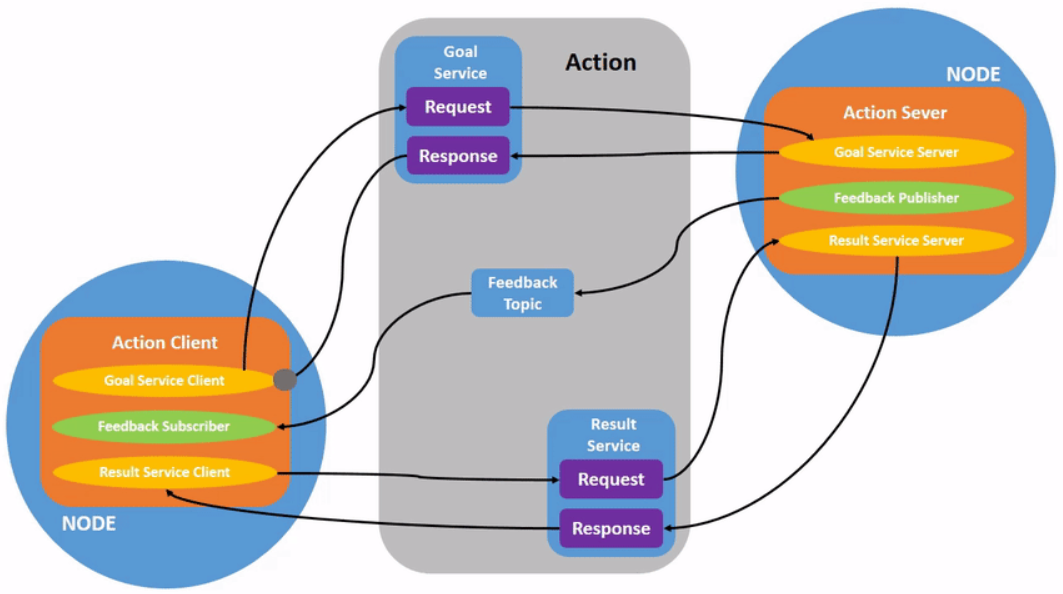
\includegraphics[width=0.8\textwidth]{c4_07.png}
    \caption{ROS2 Actions Client-Server Architecture}
    \label{fig:actions_architecture}
\end{figure}

Leveraging the ROS2 Actions client-server architecture made it possible to implement high-level tasks for the mobile manipulator
robot. The \textbf{Actions architecture} is a powerful and flexible way to define and execute complex tasks
in a distributed system, such as a robotic system composed of many nodes that need to coordinate and communicate
to perform high-level behaviors. The Actions architecture is built on top of the ROS2 middleware, which provides
a robust and reliable communication system. It allows for asynchronous communication between nodes,
enabling the robot to perform multiple tasks concurrently and efficiently. The Actions architecture is based on
the concept of goals, which represent the desired outcome of a task, and results, which represent the task's outcome.

The goal request is a non-blocking call sent by the client to the server, which executes the task asynchronously,
generating feedback messages to inform the client about the task's progress. The server sends a result message
to the client once the task is completed or aborted, indicating the outcome of the task.
The client can monitor the task's progress with the feedback messages and cancel it if necessary, providing a robust 
and reliable way to manage high-level behaviors. The advantage of using the Actions architecture is the on-demand
asynchronous execution of tasks, allowing for multiple tasks to be executed concurrently without blocking the system.
This architecture decouples the task's definition from its execution, allowing for easy code reusability and extensibility
across different applications. 

The architecture diagram of the ROS2 Actions client-server is shown in Figure \ref{fig:actions_architecture}.
The client sends a goal message to the server, which processes the goal and generates feedback messages
to inform the client about the task's progress. The server then sends a result message to the client
once the task is completed. The client can also send a cancel message to the server to stop the task
prematurely.

\begin{itemize}
    \item \textbf{ROS2 Action Server}: the servers are nodes that handle the task execution, and they are responsible
    for processing the goals, generating feedback messages, and sending the result messages to the clients.
    The servers are implemented on top of the underlying algorithms and functionalities that perform the tasks,
    provided by a separate node inside the same package.
    \item \textbf{ROS2 Action Client}: the clients are nodes that send the goals to the servers, monitor the task's progress
    with the feedback messages, and receive the result messages once the task is completed. The clients are implemented
    as unique nodes that handle the sequence of actions to be executed, decoupled from the underlying algorithms
    and instructions that perform the tasks.
\end{itemize}

The ROS2 Actions architecture is employed to implement the demonstrations explained in the sections \ref{sec:demo1} and
\ref{sec:demo2}. The high-level tasks, such as moving the robot to a specific location, and manipulating objects
or interacting with them, are implemented as Actions servers, which are called by the Actions clients to execute
the tasks. The diagrams in Figures \ref{fig:arch1} and \ref{fig:arch2} show the architecture of the implementations
of the demonstrations and how the clients and servers interact across multiple components, using the 
ROS2 middleware for communication.